\section{Vorüberlegung zur Komplexität}
\label{sec:Komplexity1}
%
\begin{floatingfigure}[hr!]{6cm}
 \centering
         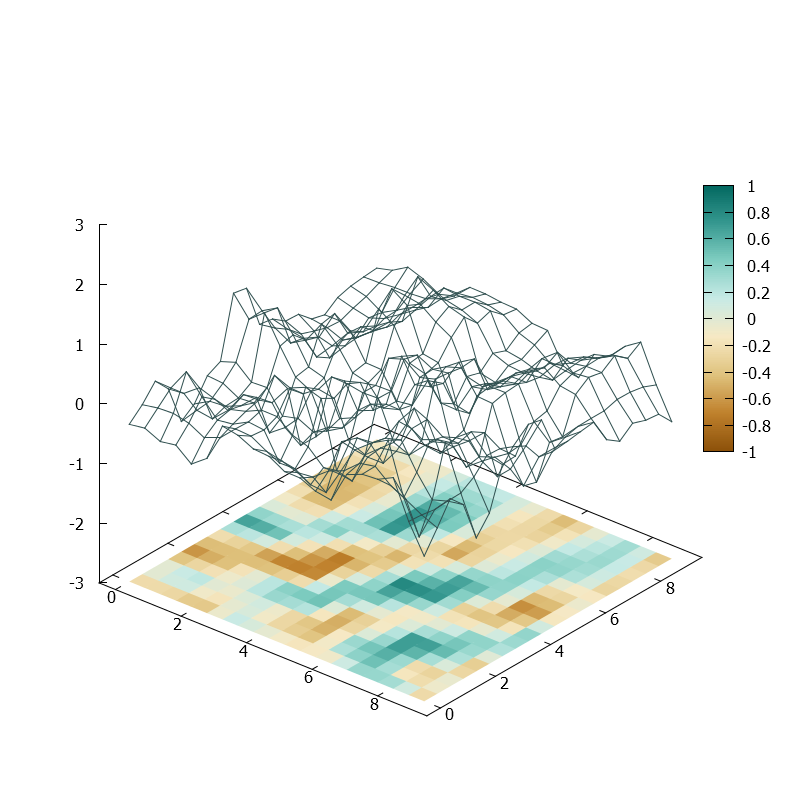
\includegraphics[width=7cm]{img/Plate0_A1.png}
         \caption[Profil einer Phasenmessung]{Normiertes Höhenprofil einer Phasenmessung aus der Sicht von Antenne 1 }
         \label{fig:Plate0_A1_}
\end{floatingfigure}
%
In diesem Abschnitt wird eine Übersicht über die Komplexität des Problems gegeben. In der rechten Abbildung zu sehen ist vergrößert Visualisierung einer typischen Kalibriermessung. Der verwendete Aufbau ist in Abbildung~\ref{fig:Spider1}. gezeigt. Er besteht aus vier Antennen die in einer Ebene angeordnet sind. Es wurde eine reproduzierbare Aufstellung verwendet (Abbildung~\ref{fig:Spider_setup1}) und eine Fläche von $1\times1$ Meter vermessen. Alle $10$ cm wurde eine Messung gespeichert. In der Abbildung kann man deutlich das Verhalten der Phasendaten sehen. Um diesen Verlauf deutlicher zu zeigen wurden die Phasenwerte normiert und als Oberfläche in den Plot gelegt. Am Boden gezeigt ist der Kontur-Plot der Werte. Zwischen den Werten wurde Interpoliert um die Nulldurchgänge deutlicher zu zeigen. Die Übersicht aus der Sicht aller Antennen ist in Abbildung~\ref{fig:Real_Measurements} gezeigt.\\
%

In der Abbildung~\ref{fig:Complexity1} werden die Daten ohne Interpolation dargestellt. Es wurden die Höhenlinien eingezeichnet. Die Anordnung der Plots soll ein Gefühl dafür vermitteln, wie die Messwerte eines Tags sich an unterschiedlichen Postionen und aus sich verschiedener Antennen verhalten.\\
%

Die Darstellung echter Messwerte lässt Rückschlüsse auf die Komplexität des Problems zu. Es ist leicht nachzuvollziehen, dass das Zusammenspiel der Messwerte eine sehr komplexe Szene ergibt. Hier dargestellt ist bereits das Verhalten bei der Verwendung von vier Antennen. Der aktuelle Messaufbau erlaubt sogar acht Antennen. Das ergibt insgesamt eine komplexe Szenerie.\\
%
\begin{figure}[ht!]
        \centering
        \begin{subfigure}[b]{0.4\textwidth}
            \centering
            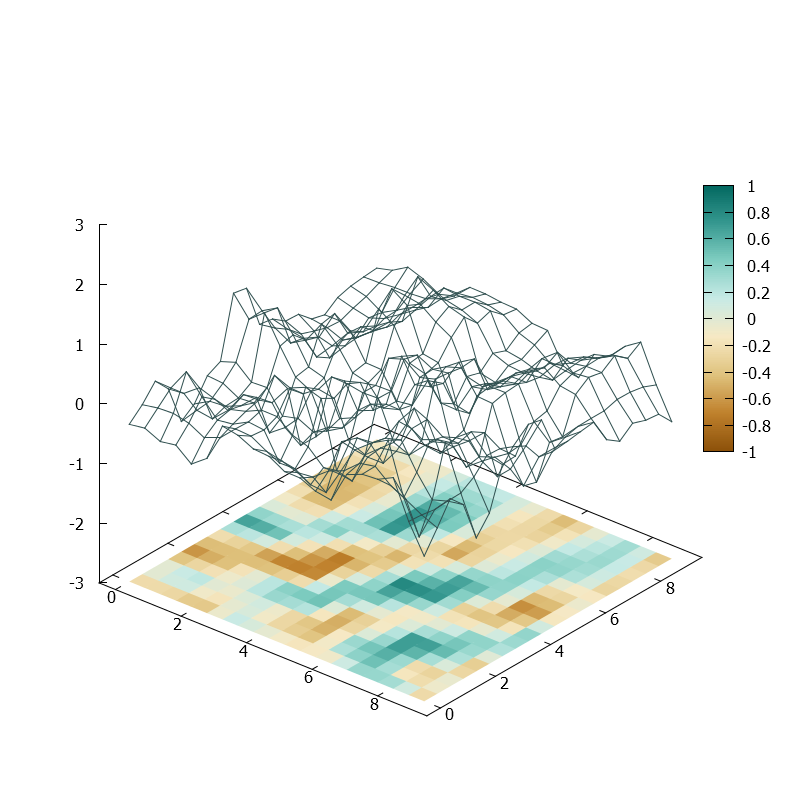
\includegraphics[width=\textwidth]{img/Plate0_A1.png}
            \caption[lorem]{Antenne 1}
            \label{fig:Plate0_A1}
        \end{subfigure}%
\\
        \begin{subfigure}[b]{0.4\textwidth}
            \centering
            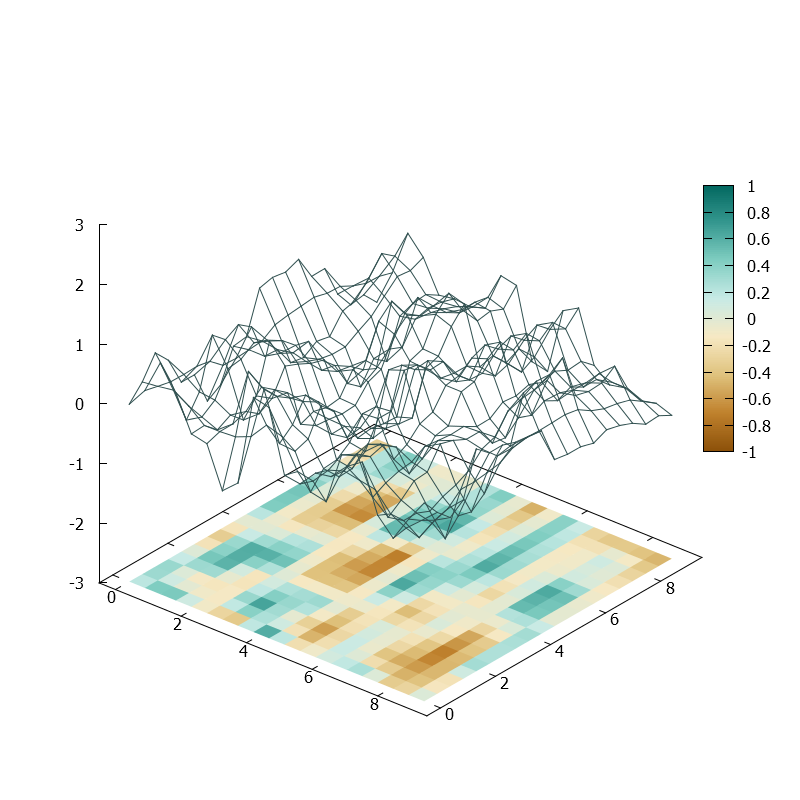
\includegraphics[width=\textwidth]{img/Plate0_A2.png}
          	\caption[Loren ipsum]{Antenne 2}
         	\label{fig:Plate0_A2}
        \end{subfigure}
\qquad\qquad
        \begin{subfigure}[b]{0.4\textwidth}
			\centering
			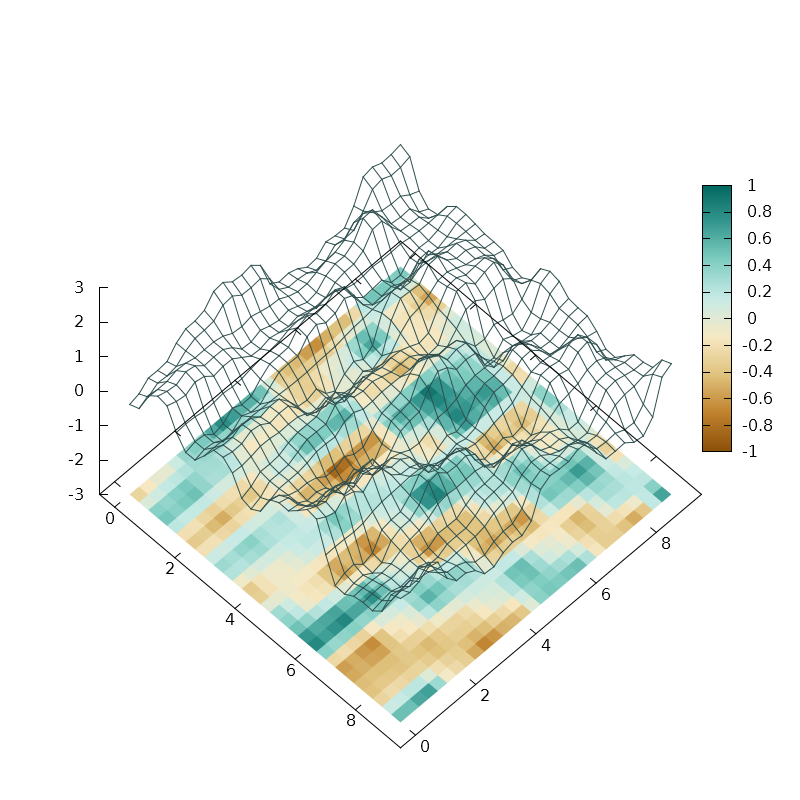
\includegraphics[width=\textwidth]{img/Plate0_A4.png}
			\caption[Loren ipsum]{Antenne 4}
			\label{fig:Plate0_A3}
        \end{subfigure}
\\
        \begin{subfigure}[b]{0.4\textwidth}
			\centering
			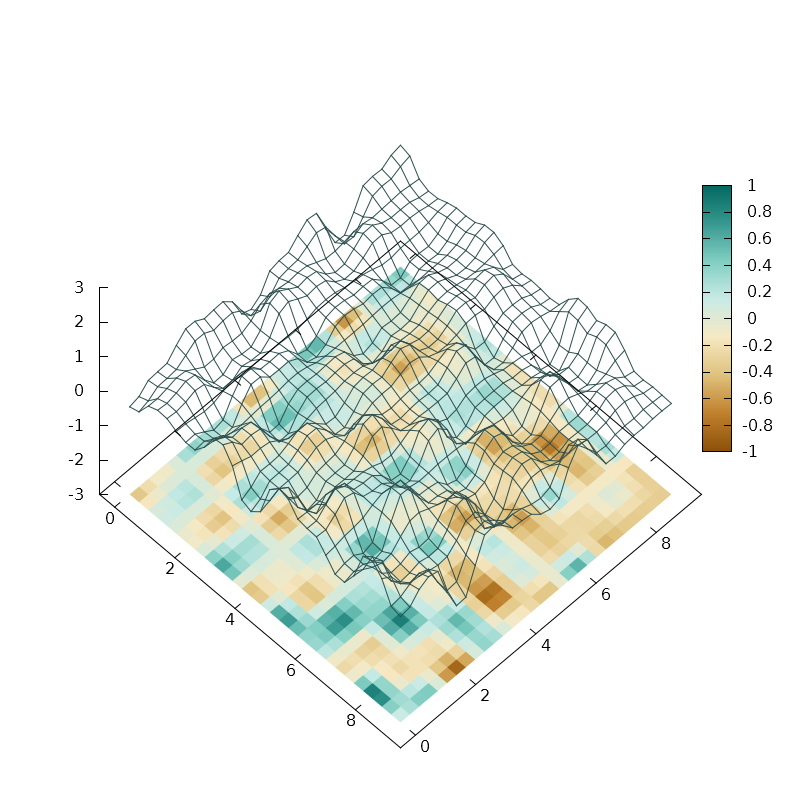
\includegraphics[width=\textwidth]{img/Plate0_A3.png}
			\caption[Loren ipsum]{Antenne 3}
			\label{fig:Plate0_A4}
        \end{subfigure}
        \caption[Reale Messwerte visualisiert]{Blick auf die Messwerte der  Kalibrierplatte aus der "Sicht" der Antennen. Dabei zeigt sich deutlich der Wellencharakter der Messung, dieser ist zu erwarten. Die Messung würden mit bei einer Frequenz von $865,7$ MHz unter Laborbedingungen aufgenommen. }\label{fig:Real_Measurements}
\end{figure}
%
\begin{figure}[ht!]
         \centering
         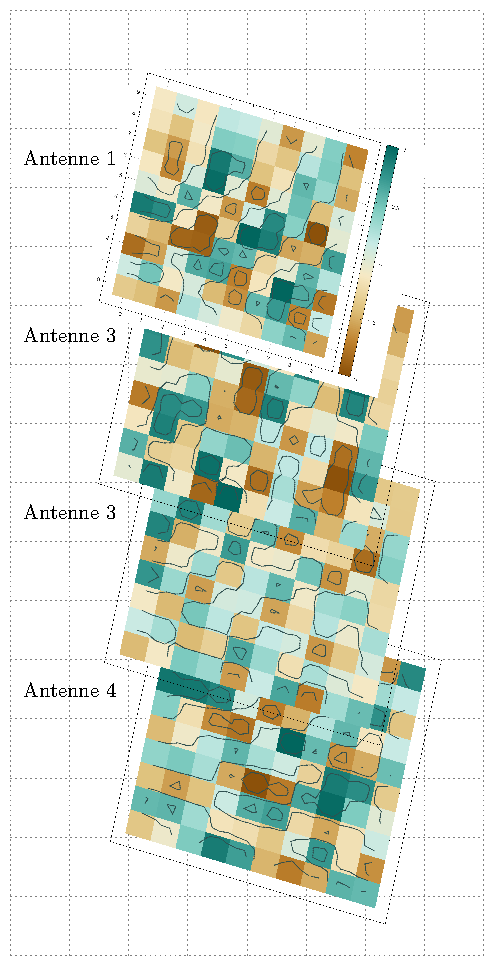
\includegraphics[width=0.6\textwidth]{img/complexitiy1.pdf}
%         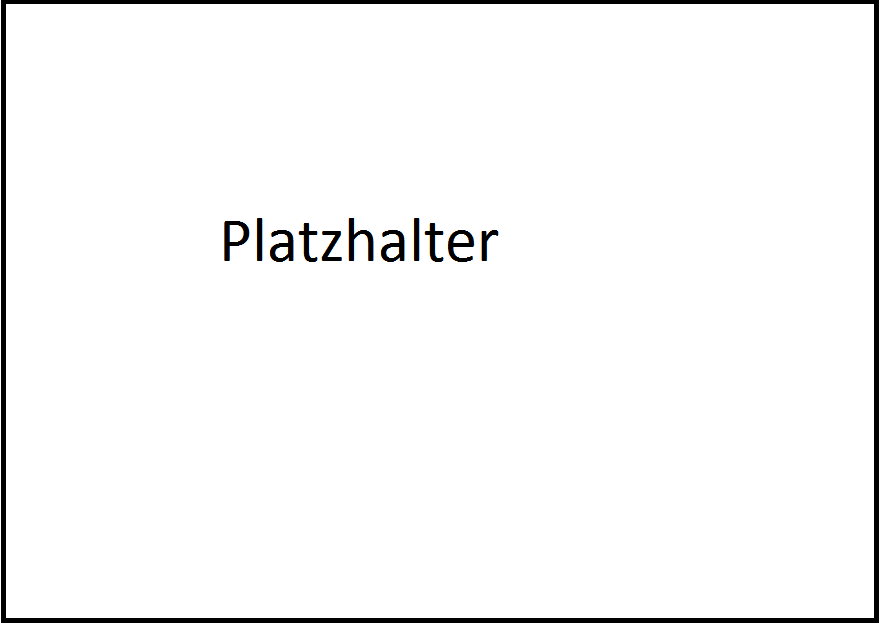
\includegraphics[width=0.7\textwidth]{img/00_placeholder.png}
         \caption[Normierte Messwerte von Kalibriermessung]{Diese Grafik zeigt die Visualisierung von realen Phasen-Messwerten. Die Daten wurden durch Vermessung einer $1\times1$-Kalibrierplatte mit reproduzierbarer Aufstellung\footnote{In dieser Arbeit nicht gezeigt} gewonnen. Die Daten wurden normiert. In jeder Dimension wurden $10\times10$ Werte aufgenommen. Die Darstellung der Phasenwerte erfolgt als Heatmap, es soll qualitativ der Verlauf der Phasenwerte gezeigt werden. Zur Orientierung sind in jedem Plot Höhenlinien eingezeichnet. Pro Plot werden die Daten einer Antenne dargestellt. Die Antenne von der die Daten stammen ist angegeben.}
         \label{fig:Complexity1}
%
\end{figure}


%
%---------------------------------------------------------------------
\section{Entwicklung des Modells}
\label{sec:model_developement}
Im folgenden Abschnitt wird das Modell für die Lösung des Zusammenhangs entwickelt. Zur Veranschaulichung des Sachverhalts dient die Abbildung~\ref{fig:TrilaterationScene}. Dort skizziert ist der Messaufbau mit einem Tag. Die Szene ist in 2D dargestellt die Ableitung des Modells erfolgt direkt für drei Raumkoordinaten.
%
\begin{figure}
	\begin{center}
		\caption[Antennen-Szene mit einem Tag]{2D-Übersicht auf die Szene mit drei Antennen, einem Tag und einer Landmarke. Die Position von $\{A_1,A_3,A_3\}$, sowie der Landmarke, zum Koordinatenursprung sind bekannt. Die Vektoren $r_1,r_2,r_3$ sind die gemessene Entfernung zu einer Antenne. Die Landmarke wird im späteren Verlauf eine Antenne sein, die ihrerseits ein gemessene Entfernung $r_0$ produziert. Der Schnittpunkt aller Kreise ist die Lösung der gemessenen Entfernung und der geom. Anordnung, die sich für die Position des Tags ergibt.} 
		\label{fig:TrilaterationScene}
		\begin{tikzpicture}[
    scale=1,
    axis/.style={thick, ->, >=stealth'},
%    vector/.style={thick, ->,-latex, >=stealth'},
%    antenna/.style={thick},
     important line/.style={thick},
     antenna/.style={thick, cyan!70},
%    dashed line/.style={dashed, thin},
%    pile/.style={thick, ->, >=stealth', shorten <=2pt, shorten
%    >=2pt},
%    every node/.style={color=black},
%    main node/.style={circle,fill=blue!20,draw},
%    help lines/.style={gray,very thin}
    ]
    % axis
    \draw[axis] (-.1,0)  -- (1,0) node(xline)[right] {$x$};
    \draw[axis] (0,-.1) -- (0,1) node(yline)[above] {$y$};

	\draw[gray, very thin, dotted] (0,0) grid (15,6);

	\coordinate (A1_start) at (4,3);
	\coordinate (A1_end) at (4,4);
	\coordinate (A2_start) at (7,5);
	\coordinate (A2_end) at (8,5);
	\coordinate (A3_start) at (8,1);
	\coordinate (A3_end) at (8,2);

	\coordinate (A1_end_) at ($(A1_start)!1!-10:(A1_end)$);
	\coordinate (A2_end_) at ($(A2_start)!1!-10:(A2_end)$);
	\coordinate (A3_end_) at ($(A3_start)!1!-35:(A3_end)$);
	
	\coordinate (Tag_0) at (6,2);
	\coordinate (REF_0) at (12,5);
	\coordinate (Int1) at ($(A1_start)!.5!(A1_end_)$);
	\coordinate (Int2) at ($(A2_start)!.5!(A2_end_)$);
	\coordinate (Int3) at ($(A3_start)!.5!(A3_end_)$);
	
	\begin{scope}
		\node [draw,orange!50,dashed] at (Int1) [circle through={(Tag_0)}] {};
		\node [draw,orange!50,dashed] at (Int2) [circle through={(Tag_0)}] {};
		\node [draw,orange!50,dashed] at (Int3) [circle through={(Tag_0)}] {};
	\end{scope}
	
	\draw[antenna] (A1_start) node[font=\scriptsize,black,below] {$A_1$} -- ($(A1_start)!1!-10:(A1_end)$);
	\draw[antenna] (A2_start) node[font=\scriptsize,black,above] {$A_2$}-- ($(A2_start)!1!-10:(A2_end)$);
	\draw[antenna] (A3_start) node[font=\scriptsize,black,below] {$A_3$}-- ($(A3_start)!1!-35:(A3_end)$);
	
	\node [green!60!black!90, right,font=\scriptsize ] at (REF_0) {$\text{Landmarke}@(x_0,y_0,z_0)$};

	\draw[latex-latex] (Tag_0) -- node[sloped,above,midway] {$r_1$}(Int1);
	\draw[latex-latex] (Tag_0) -- node[sloped,above,midway] {$r_2$}(Int2);
	\draw[latex-latex] (Tag_0) -- node[sloped,above,midway] {$r_2$}(Int3);
	\draw[-latex,dashed,green!60!black!90] (REF_0) -- node[sloped,above,midway] {$r_0$}(Tag_0);
	
	\draw[ -latex,violet!60,font=\scriptsize,dotted] (REF_0) -- node[sloped,above,midway] {$d_{10}$}(Int1);
	\draw[ -latex,violet!60,font=\scriptsize,dotted] (REF_0) -- node[sloped,above,midway] {$d_{20}$}(Int2);
	\draw[ -latex,violet!60,font=\scriptsize,dotted] (REF_0) -- node[sloped,above,midway] {$d_{30}$}(Int3);
		
	\fill[red!70] (Tag_0) circle [radius=2pt];
	\node[font=\scriptsize,black,below] at (Tag_0) {$Tag$} ;
	\fill[green!60!black!90] (REF_0) circle [radius=2pt];
	
\end{tikzpicture}



%		
	\end{center}
\end{figure}
%
Folgende Nomenklatur und Symbole gelten für diesen Abschnitt:
\begin{itemize}[itemsep=0mm]
	\item	$r_{k}$ := Abstand vom Tag zur Antenne
	\item	$d_{kJ}$ := Abstand zur Landmarke
	\item	$N_0:=$ Menge der verfügbaren Antennen $N=\{1,..,8\}$
	\item	$N:=$ Menge der Antennen die für die Optimierung verwendet werden können ($N \subseteq N_0$)
	\item	$N':=$ Menge der Antennen die für die Optimierung verwendet werden ($N' \subseteq N$)
%	; Dabei ist $|N'| \geq 3$
%	\item	Es gilt $|N'| \geq |N| \geq |N_0|$   
	\item	$j$ ist der Index der Referenzantenne, es gilt $j = \{1,2,..,8\}$
	\item	$k$ ist der Index der Antennen einer Messung, es gilt $k = 1,2,..,|N'|-1$
\end{itemize}
%
Wir starten mit der Überlegung über den geometrischen Zusammenhang zwischen der Antennenposition von Antenne $k$ zu der Position des Tags $r_k$:
\begin{align}
	\label{eq:base_vactor}
	r_{k}^2 &= (x-x_k)^2+(y-y_k)^2+(z-z_k)^2
\end{align}
%
Diese Gleichung stellt die Euklidische Vektornorm dar und entspricht der Strecke Antenne-Tag. Für die Ermittelung einer Postion (mit drei Raumkoordinaten) sind drei Antennen Notwendig. Daraus ergibt sich:
%
\begin{itemize}
\item 3 Gleichunge n
\item 3 Unbekannte
\item Quadratisches Gleichungssystem
\end{itemize}
%
Das Gleichungssystem sieht wie folgt aus:
%
\begin{align}
	r_{1}^2 &= (x-x_1)^2+(y-y_1)^2+(z-z_1)^2 \nonumber\\
	r_{2}^2 &= (x-x_2)^2+(y-y_2)^2+(z-z_2)^2 \nonumber\\
	r_{3}^2 &= (x-x_3)^2+(y-y_3)^2+(z-z_3)^2 \nonumber
%	
\end{align}
%
Es ist trivial und wird in verschiedenen Beispielen gezeigt\footnote{z.B. \url{http://en.wikipedia.org/w/index.php?title=Trilateration&oldid=553215995}}, dass man die Koordinaten aus dem quadratischen Gleichungssystem unmittelbar berechnen kann. Es muss jedoch ein quadratisches Gleichungssystem gelöst werden, was zu den bekannten Problematiken führt, insbesondere der Ausschluss mehrdeutiger Ergebnisse. Der Messaufbau der \amedogmbh erlaubt die Verwendung von mehr als 3 Messwertgebern. Diese zusätzliche Informationen lassen sich für eine Linearisierung des Gleichungssystems verwenden. Dieser Ansatz wird für ein Modell im Rahmen dieser Arbeit verwendet und wird im Folgenden beschrieben.\\
%
Von den Antennen sind die Raumkoordinaten ($x,y,z-Koordinaten$) bekannt, bzw. wurden durch Kalibrierung \ref{sec:calibration} in einem vorherigen Schritt bestimmt. Wir können zusätzlich zu notieren:
%
\begin{equation}\label{eq:d_k0}
	d_{kj}^2= (x_k-x_0)^2+(y_k-y_0)^2+(z_k-z_0)^2
\end{equation}
%
Linearisierung des Modells. Dazu wird Gleichung~\ref{eq:base_vactor} in mehreren Schritten umgebaut. Zuerst wird eine neutrale Erweiterung durchgeführt und die Terme geschickt zusammengefasst. Das führt zu:
%
\begin{align}
	r_{k}^2 &= (x-x_k)^2+(y-y_k)^2+(z-z_k)^2 \nonumber \\
	&=(x-x_k+x_0-x_0)^2+(y-y_k+y_0-y_0)^2+(z-z_k+z_0-z_0)^2 \nonumber \\
	&=((x-x_0)-(x_k-x_0))^2+((y-y_0)-(y_k-y_0))^2+((z-z_0)-(z_k-z_0))^2 \nonumber \\ 
	%2 bin. Form
	&=(x-x_0)^2-2(x-x_0)(x_k-x_0)+(x_k-x_0)^2\underbrace{+\dots{}+\dots{}}_\text{y-\& z-Terme analog}
	\label{eq:tri_temp1}
%
\end{align}
%
Um Platz zu sparen sind die y- und z-Terme nicht explizit notiert. Sie ergeben sich durch einfaches Ersetzen der Indizes und werden im Finalen Modell eingefügt. Durch Umstellen von \eqref{eq:tri_temp1} erhalten wir:
\begin{align}
(x-x_0)(x_k-x_0)+\dots{}+\dots{}&=-\frac{1}{2}[r_k^2-(x_k-x_0)^2 -(x-x_0)^2 +\dots{} +\dots{}]\nonumber\\
(x-x_0)(x_k-x_0)+\dots{}+\dots{}&=\phantom{-}\frac{1}{2}[(x_k-x_0)^2 +(x-x_0)^2 +\dots{}+\dots{}-r_k^2]\nonumber
%
\end{align}
%
\begin{multline}\label{eq:rk_final}
(x-x_0)(x_k-x_0)+(y-y_0)(y_k-y_0)+(z-z_0)(z_k-z_0)= \\\frac{1}{2}[(x_k-x_0)^2+(x-x_0)^2-(y_k-y_0)^2+(y-y_0)^2
\\-(z_k-z_0)^2 +(z-z_0)^2-r_k^2]
\end{multline}
%
Vergleich von \eqref{eq:rk_final} mit \eqref{eq:d_k0} bringt: 
%
\begin{multline}
(x-x_0)(x_k-x_0)+(y-y_0)(y_k-y_0)+(z-z_0)(z_k-z_0)= \\\frac{1}{2}[\underbrace{(x_k-x_0)^2+(z_k-z_0)^2+(y_k-y_0)^2}_\text{\boldmath{$d_{kj}^2$}}
\\+\underbrace{(x-x_0)^2+(y-y_0)^2 +(z-z_0)^2}_\text{\boldmath{$r_j^2$}}-r_k^2]
\end{multline}
%
\begin{equation}
(x-x_0)(x_k-x_0)+(y-y_0)(y_k-y_0)+(z-z_0)(z_k-z_0)=\frac{1}{2}[d_{kj}^2+r_{j}^2-r_k^2]\label{eq:rk_final_simplyfied}
\end{equation}
mit 
\begin{equation}\label{eq:c_kj}
\mathbf{c_{kj}}=\frac{1}{2}[d_{kj}^2+r_{j}^2-r_k^2]
\end{equation}
können wir das lineare Gleichungssystem abschließend schreiben:
%
\begin{equation}
%\label{eq:final_trilateration_model}
\mathbf{0}=
\left(
	\begin{array}{ccc}
		x_1-x_j & y_1-y_j & z_1-z_j \\
		x_2-x_j & y_2-y_j & z_2-z_j \\
		x_3-x_j & y_3-y_j & z_3-z_j
	\end{array}
\right)
\left(
   \begin{array}{c}
	   x-x_j\\
	   y-y_j\\
	   z-z_j
   \end{array}
\right)
-
\left(
	\begin{array}{c}
		c_{1j}\\
		c_{2j}\\
		c_{3j}
	\end{array}
\right)
\end{equation}
%
Das Gleichungssystem entspricht ist linear und hat die allg. Form: $\mathbf{0} = \mathbf{Ax}+\mathbf{b}$ es lässt sich mit bekannten Methoden lösen.




{
\small
Folgende Nomenklatur und Symbole gelten für diesen Abschnitt:
%
Wie gezeigt werden konnte\footnote{Wochenbericht KW 20, Anhang B} ergibt sich für den Fall der Trilateration und der Annahme, dass vier Antennen Messwerte liefern, die Gleichung:
\begin{equation}\label{eq:final_trilateration_model}
0=
\left(
	\begin{array}{ccc}
		x_k-x_0 & y_k-y_0 & z_k-z_0 
	\end{array}
\right)
\left(
   \begin{array}{c}
	   x-x_0\\
	   y-y_0\\
	   z-z_0
   \end{array}
\right)
-
\left(
	\begin{array}{c}
		c_{kj}
	\end{array}
\right) 
\end{equation}
%
Dabei ist:
\begin{equation}\label{eq:c_kj}
	c_{kj}=\frac{1}{2}[d_{kj}^2+r_{j}^2-r_k^2]
\end{equation}
%
Ziel dieser Erweiterung ist es, einen Zusammenhang zwischen diesem Modell und der Wellenzahl zu erzeugen. Folgender Ansatz wird gewählt:
	\begin{equation}\label{eq:r_0_varrho} r(\varrho)=\frac{\lambda}{2}\left(\frac{\varrho}{2\pi}+n\right),\\\lambda=\frac{c}{f}, n:= \text{Wellenzahl}
\end{equation}
%
%
Weiterhin ist $\varrho$ die gemessene Phase, die das PRPS-System liefert und $n$ die gesuchte Wellenzahl.\\
Durch einsetzen von \eqref{eq:r_0_varrho} in \eqref{eq:c_kj}, erhalten wir:
\begin{equation}\label{eq:c_k0_extended}
	c_{kj}(\varrho_0, \varrho_k, n_0, n_k) =\frac{1}{2}\left[d_{kj}^2+\frac{\lambda^2}{4}\left(\frac{\varrho_j}{2\pi}+n_0\right)^2-\frac{\lambda^2}{4}\left(\frac{\varrho_k}{2\pi}+n_k\right)^2\right]
\end{equation}
%
Wir stellen Gleichung~\eqref{eq:c_k0_extended} um:
\begin{align}
%	
	c_{kj}(\varrho_0, \varrho_k, n_0, n_k) &= \frac{1}{2}\left\{d_{kj}^2+\frac{\lambda^2}{4}\left[\left(\frac{\varrho_j}{2\pi}\right)^2+2\frac{\varrho_j}{2\pi}n_0+n_0^2 \right.\right.\nonumber\\
	&\phantom{=}\; 
	\left.\left.-\left(\frac{\varrho_k}{2\pi}\right)^2-2\frac{\varrho_k}{2\pi}n_k-n_k^2\right]\right\}\\
%    
    &=\frac{1}{2}\left\{d_{kj}^2+\frac{\lambda^2}{4}\left[\left(\frac{\varrho_j}{2\pi}\right)^2-\left(\frac{\varrho_k}{2\pi}\right)^2 \right.\right.\nonumber\\
    &\phantom{=}\;
   	\left.\left.+2\frac{\varrho_j}{2\pi}n_0-2\frac{\varrho_k}{2\pi}n_k+n_0^2-n_k^2\right]\right\}\\
%	
	&=\frac{1}{2}d_{kj}^2+\frac{\lambda^2}{8}\left[\frac{1}{(2\pi)^2}\left(\varrho_0^2-\varrho_k^2\right) \right.\nonumber\\
	&\phantom{=}\;
	\left. +\frac{1}{\pi}\left(\varrho_0n_0-\varrho_kn_k\right)+\left(n_0^2-n_k^2\right)\right]\label{c_k0_rearragend}
\end{align}
%
Führen wir nun:
\phantomeq{c_{kj}(\varrho_0, \varrho_k, n_0, n_k)}{a_{0k} := \frac{1}{2}d_{kj}^2\nonumber}
\phantomeq{c_{kj}(\varrho_0, \varrho_k, n_0, n_k)}{a_1 := \frac{\lambda^2}{8}\nonumber}
\phantomeq{c_{kj}(\varrho_0, \varrho_k, n_0, n_k)}{a_2 := a_1\frac{1}{\pi}\nonumber}
\phantomeq{c_{kj}(\varrho_0, \varrho_k, n_0, n_k)}{a_{3kj} := a_1\frac{1}{(2\pi)^2}(\varrho_j^2-\varrho_k^2)\nonumber}
%
in Gleichung~\eqref{c_k0_rearragend} ein, erhalten die finale Form der Gleichung:
\begin{equation}
c_{kj}(\varrho_0, \varrho_k, n_0, n_k) = a_{0k}+a_1(n_0^2-n_k^2)+a_2(\varrho_0n_0-\varrho_kn_k)-a_{3kj}\label{c_k0_final_form}   
\end{equation}
%
Die Einführung der Konstanten macht zum Einen die Gleichung übersichtlicher. Zum Anderen können so, mit Blick auf eine spätere Softwareimplementation, Rechenschritte gespart werden. Das sollte sich positiv auf den späteren Berechnungsaufwand auswirken.\\
%
Im Weiteren erkennt man durch scharfes hinsehen das in Gleichung~\eqref{c_k0_final_form}, für $\varrho_k=\text{const.}$ \& $\varrho_0=\text{const.}$ gilt. Das resultiert aus der Tatsache, dass . Es ermöglicht uns zu schreiben:
\begin{equation}
c_{kj}(\varrho_0, \varrho_k, n_0, n_k) = c_{kj}(n_0, n_k)
\end{equation}
%
Im engeren Sinne einer mathematischen Funktion sollten wir die Parameter alle als Argument aufnehmen. Diese Form soll darstellen, welche Größen von Interesse sind. Im späteren Gebrauch wird diese Gleichung in der Optimierung eingesetzt werden.
Für unser Gleichungssystem aus\eqref{eq:final_trilateration_model} ergibt sich:
\begin{equation}\label{eq:wavenumber_trilateration_model}
0=
\left(
	\begin{array}{ccc}
		x_k-x_0 & y_k-y_0 & z_k-z_0 
	\end{array}
\right)
\left(
   \begin{array}{c}
	   x-x_0\\
	   y-y_0\\
	   z-z_0
   \end{array}
\right)
-
\left(
	\begin{array}{c}
		c_{kj}(n_0, n_k)
	\end{array}
\right)
\end{equation}
%
Betrachten wir nun \eqref{eq:wavenumber_trilateration_model}, wählen $N'=4$ (d.h. wir verwenden 4 Antennen) und setzen $j=0$. Wir beschreiben die Konfiguration wie folgt: Antenne 0 ist die Referenz-Antenne und Antenne 0-3 sind Messwertgeber für die Phaseninformation. 
%
\begin{equation}\label{eq:wavenumber_trilateration_model_explicit}
0=
\underbrace{\left(
	\begin{array}{ccc}
		x_1-x_0 & y_1-y_0 & z_1-z_0 \\
		x_2-x_0 & y_2-y_0 & z_2-z_0 \\
		x_3-x_0 & y_3-y_0 & z_3-z_0 
	\end{array}
\right)}_{\textbf{A}}
\underbrace{\left(
   \begin{array}{c}
	   x-x_0\\
	   y-y_0\\
	   z-z_0
   \end{array}
\right)}_{\textbf{x}}
-
\underbrace{\left(
	\begin{array}{c}
		c_{10}(n_0, n_1) \\
		c_{20}(n_0, n_2) \\
		c_{30}(n_0, n_3)
	\end{array}
\right)}_{\textbf{b}}
\end{equation}
%
\begin{equation}
\mathbf{b}=
\left(
	\begin{array}{c}
		a_{01}+a_1( n_0^2-n_1^2)+a_2(\varrho_0n_0-\varrho_1n_1)-a_{310} \\
		a_{02}+a_1(n_0^2-n_2^2)+a_2(\varrho_0n_0-\varrho_2n_2)-a_{320} \\
		a_{03}+a_1(n_0^2-n_3^2)+a_2(\varrho_0n_0-\varrho_3n_3)-a_{330}
	\end{array}
\right)
\end{equation}
%
Das Ergebnis ist ein um $\varrho$ und $n$ erweitertes Gleichungssystem. Zusätzlich enthält  es mehrere geometrische Konstanten ($a_{0k}, k=\{1,..,N-1\}$), mehrere Phasen-Konstanten ($a_{3k0}, k=\{1,..,N-1\}$), sowie zwei allgemeine ($a_1$ und $a_2$). Allgemeiner formuliert ergibt sich:
%
\begin{multline}\label{eq:final_equation}
0=
\left(
	\begin{array}{ccc}
		x_k-x_0 & y_k-y_0 & z_k-z_0 
	\end{array}
\right)
\left(
   \begin{array}{c}
	   x-x_0\\
	   y-y_0\\
	   z-z_0
   \end{array}
\right) \\
-
\left(
	\begin{array}{c}
		a_{0k}+a_1(n_0^2-n_k^2)+a_2(\varrho_0k_0-\varrho_kn_k)-a_{3kj}
	\end{array}
	\right)
\end{multline}
%
Aus Gleichung~\eqref{eq:final_equation} ist durch eine geeignete Wahl von $N'=\{4,..,N\}$ sofort ersichtlich wie viele Veränderliche sich für eine gewählte Konstellation an Antennen ergeben. Für $k$ gilt in diesem Fall $k=\{1,..,N'-1\}$.\\
%
Beispielsweise ergibt sich für das Modell aus Gleichung~\eqref{eq:final_equation} mit $N'=4$, insgesamt 7 Variablen ($\mathbf{x},n_0,n_1,n_2,n_3$) . Analog würde sich für ein Modell mit allen 8 Antennen, 11 Variablen ($\mathbf{x},n_0,..,n_7$) ergeben.
}
{
Abschließend soll das das bisher verwendete Modell umgeschrieben werden, damit die Allgemeingültigkeit darin enthalten ist.
\begin{align}
%
%\mathbf{0}&=\mathbf{A}\mathbf{x}-\mathbf{b}\\
%
\mathbf{A}&=
\left(
	\begin{array}{cccccc}
		x_k-x_0 & y_k-y_0 & z_k-z_0 & \sum_{i=1,j=0}^{k}(-a_1\delta_{ij}) &  -a_2\Theta_0 & \sum_{i=1,j=0}^{k}(a_2\Theta_k\delta_{ij})
	\end{array}
\right)\nonumber\\
%
\mathbf{x}&=
\left(
   \begin{array}{c}
	   x-x_0\\
	   y-y_0\\
	   z-z_0\\
	   n_0^2-n_k^2\\
	   n_0\\
	   n_k
   \end{array}
\right)\nonumber\\
%
\mathbf{b}&=
	\begin{array}{c}
		a_{0k}-a_{3kj} 
	\end{array}
	= c_{kj}'\nonumber
\end{align}
%
Dabei steht $\delta_{ij}$ für den bekannten Kronecker-Operator und bedeutet:
\begin{equation*}
\delta_{ij} = \begin{cases}1 ~\text{für}~ i=j\\ 0 ~\text{für}~ i\neq j\end{cases}
\end{equation*}
%
Im Expliziten sehen die Matrix $\mathbf{A}$ und der Vektor $\mathbf{b}$, für denn Fall $N'=3$ und $k=\{1,2,3\}$, wie folgt aus:
%
\begin{multline}
\mathbf{A}=\\
\left(
	\begin{array}{cccccccccc}
		x_1-x_0 & y_1-y_0 & z_1-z_0 & -a_1 & 0 & 0 & -a_2\Theta_0 & a_2\Theta_3 & 0 & 0 \\
		x_2-x_0 & y_2-y_0 & z_2-z_0 & 0 & -a_1 & 0 & -a_2\Theta_0& 0 & a_2\Theta_3 & 0 \\
		x_3-x_0 & y_3-y_0 & z_3-z_0 & 0 & 0 & -a_1 & -a_2\Theta_0& 0 & 0 & a_2\Theta_3
	\end{array}
\right) \nonumber
\end{multline}
%
\begin{equation}
\mathbf{x}=
\left(
	\begin{array}{c}
		x-x_0	\\
		y-y_0	\\
		z-z_0	\\
		n_0^2-n_1^2	\\
		(\dots)	\\
		n_0^2-n_3^2	\\
		n_0 \\
		n_1	\\
		(\dots)	\\
		n_3	
	\end{array}
\right)\nonumber
\end{equation}
%
\subsubsection{Bemerkungen - Finales Modell}
%
Das Ergebnis ist eine $3\times10$ Matrix und ein $1\times10$ Vaktor. Es ist möglich diesem Modell eine beliebige Anzahl an Antennen hinzuzufügen. Fügt man eine Antenne zur Berechnung hinzufügen würde sich die Matrix $\mathbf{A}$ um zwei Spalten und eine Zeile erweitern, der Vektor $\mathbf{x}$ analog um 2 Zeilen.

}

%
%---------------------------------------------------------------------
\section{Antennen Permutationen}
%
\begin{figure}[hr!]
	\begin{center}
		\caption[Ablauf libPermuatate]{ lorem }
		\label{fig:libpermutate_flowchart}
		\vspace{0.5cm}
		\begin{tikzpicture}[scale=.3]
		\scriptsize
			\tikzstyle{decision} = [diamond, draw=black, thick, fill=black!20, text width=5em, text badly centered, inner sep=1pt]
%			
			\tikzstyle{block} = [rectangle, draw=black, thick, fill=gray!20, text width=15em, text centered, rounded corners, minimum height=4em]
%	
			\tikzstyle{line} = [draw, thick, -latex',shorten >=1pt];
			\tikzstyle{commentline} = [draw, dashed, green!50,-latex',shorten >=1pt];
%	
			\tikzstyle{cloud} = [ dotted, draw=green!50, thick, ellipse,,fill=green!20, minimum height=2em, text width= 10em, text badly centered];
%	
			\matrix [column sep=5mm,row sep=7mm]
			{
				% row 1
				& \node [block] (start) { Start }; & \\
				% row 2
				&\node [block] (read) { Lese Koordinaten aus der Datei }; &\\
				% row 4
				& \node [block] (calcPermutations) {Berechne Permutationen}; & \\
				%				
				& \node [block] (calcMatrixes) {Berechne Matrizen}; & \\	
				% row 5
				& \node [block] (store) {Speichere die Konfigurationen in entsprechender Struktur}; & \\
				%				
				& \node [block] (write) {Schreibe Konfigurationen in CSV-Datei}; & \\
				% row 6
				& \node [block] (stop) {Ende}; & \\
			};
% Arrows
			\tikzstyle{every path}=[line]
			\path (start) -- (read);
			\path (read) -- (calcPermutations);
			\path (calcPermutations) -- (calcMatrixes);
			\path (calcMatrixes) -- (store);
			\path (store) -- (write);
			\path (write) -- (stop);
			
		\end{tikzpicture}
	\end{center}
\end{figure}
%
Um die Beurteilung der Konditionszahl der Matrizen effizient durchführen zu können, wurde im Rahmen dieser Arbeit ein Programm geschrieben. Es erstellt automatisch, auf Basis der durch die Kalibrierung bestimmten Koordinaten, alle möglichen Permutationen von Antennen. Die sich ergebenden Matrizen sind immer auf eine Referenzantenne bezogen. Es ergeben sich, bezogen auf eine Referenzantenne, folgende Anzahl an Matrizen:
% 
\begin{equation}
	\frac{7!}{3!(7-3)!}=35
% 
\end{equation}
%Wdh, steht oben schon: Die sich ergebenen Matrizen sind immer auf eine Referenzantenne bezogen. Es ergeben sich für eine Referenzantenne folgende Anzahl an Matrizen:
%
Für einen Aufbau mit acht Antennen ergeben sich so $8\times 35 = 280$ mögliche Anordnungen. Die Implementation der Berechnungen der Permutationen findet sich in dem Modul \textit{'libPermutate'}. Das Modul generiert bei der Instanziierung automatisch alle möglichen Kombinationen von Antennen und speichert diese in einer geeigneten Struktur für den späteren Gebrauch. Das Ablaufdiagramm ist in Abbildung~\ref{fig:libpermutate_flowchart} zu finden.\\
%
%\begin{equation}
%\frac{7!}{3!(7-3)!}=35
%\end{equation}
%%
%Insgesamt ergeben sich so $8\times 35 = 280$ mögliche Anordnungen. Das erstellte Tool soll in ein entsprechendes C++-Programm portiert werden. Diese Berechnungen werden im späteren System auf jeden Fall anfallen.




%
%---------------------------------------------------------------------
\section{Erweiterte Betrachtung der Kondition}
%
Die vorgestellte erweiterte Form des Modells erleichtert Implementation und Verifikation. Große Teile des Modells sind statisch (vgl. \ref{eq:block_matrix_form}) und können im Voraus berechnet werden. Es sind nun auch die gemessenen Phasenwerte Teil des Modells, genauer: der Matrix $\mathbf{A}$. Im Folgenden werden die Auswirkungen auf die Kondition der Matrix betrachtet. Dazu wird Untersucht inwieweit die Zerlegung in Blockmatrizen und die Untersuchung der Kondition dieser eine Abschätzung der vollständigen Konditionszahl im Allgemeinen darstellt. 
%
\begin{equation}
\label{eq:block_matrix_form}
\mathbf{A}=\bigg( \mathbf{Z}\quad \mathbf{P}\quad \mathbf{V}\bigg)
\end{equation}
%
Dabei ist:
\begin{equation}
\mathbf{Z} \in \mathbb{R}^{3x3} \quad \mathbf{P} \in \mathbb{R}^{3x3} \quad \mathbf{V}\in \mathbb{R}^{4x3}
\end{equation}
%
Die Matrizen $\mathbf{Z}$ und $\mathbf{P}$ sind statisch. Hingegen enthält die Matrix $\mathbf{V}$ die gemessenen Phasenwerte $\Theta_k$ der Antennen für diese Konfiguration. \\
%
Die Abbildung~\ref{fig:CondNumberAnalyze} zeigt die bereits angestellte Untersuchung zu dieser Überlegung. Abbildung~\ref{fig:AnalyzeOf3x3} stellt die Konditionszahl der rein geometrischen $3\times3$-Matrix dar. In der Abbildung~\ref{fig:AnalyzeOf10x3} sehen wir die Kondition der erweiterten Matrix. Neben der geometrischen sind auch die beiden anderen Blockmatrizen in diese Konditionsbetrachtung eingeflossen. Als zusätzliche Angabe wird ist sind die Skalierungsfaktoren angegeben. Legt man beide Grafiken übereinander erkennt man:
\begin{enumerate}
\item Geometrisch gut konditionierte Konfigurationen (linke Grafik), bleiben im erweiterten Modell (rechte Grafik) weiterhin gut konditioniert.
\item Die Konditionszahl der \textit{schlechteste} ist wesentlich kleiner (ca. Faktor $10$) als im rein geometrischen Modell
\end{enumerate}
%
\begin{figure}[h]
         \centering
	     \caption{Analyse der Konditionszahlen aller möglichen Matrizen für den Messaufbau; Die Konditionszahl ist für jede mögliche Permutation an Messantennen für eine Referenzantenne angegeben}\label{fig:CondNumberAnalyze}
         \begin{subfigure}[h]{0.5\textwidth}
                 \centering
                 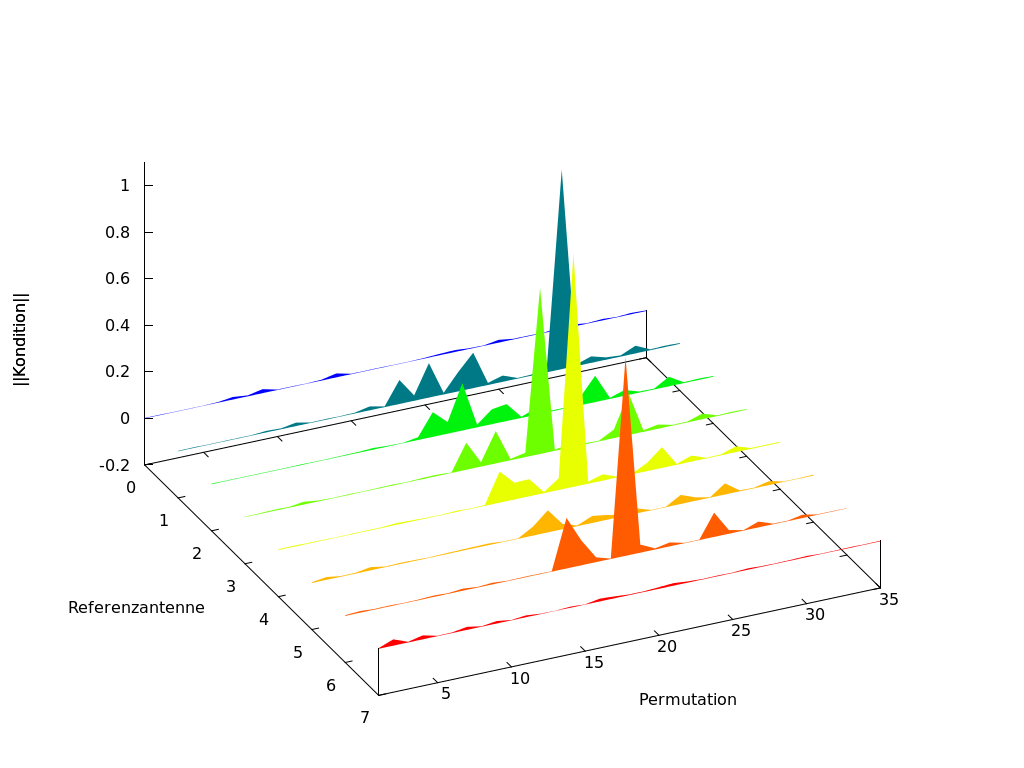
\includegraphics[width=\textwidth]{img/fenceModell3x3.png}
                 \caption{Konditionszahl der rein geometrischen $3\times3$ Matrix normiert auf den größten vorkommenden Wert ($=2149,16                 $)}
                 \label{fig:AnalyzeOf3x3}
         \end{subfigure}
%         
         \begin{subfigure}[h]{0.5\textwidth}
                 \centering
                 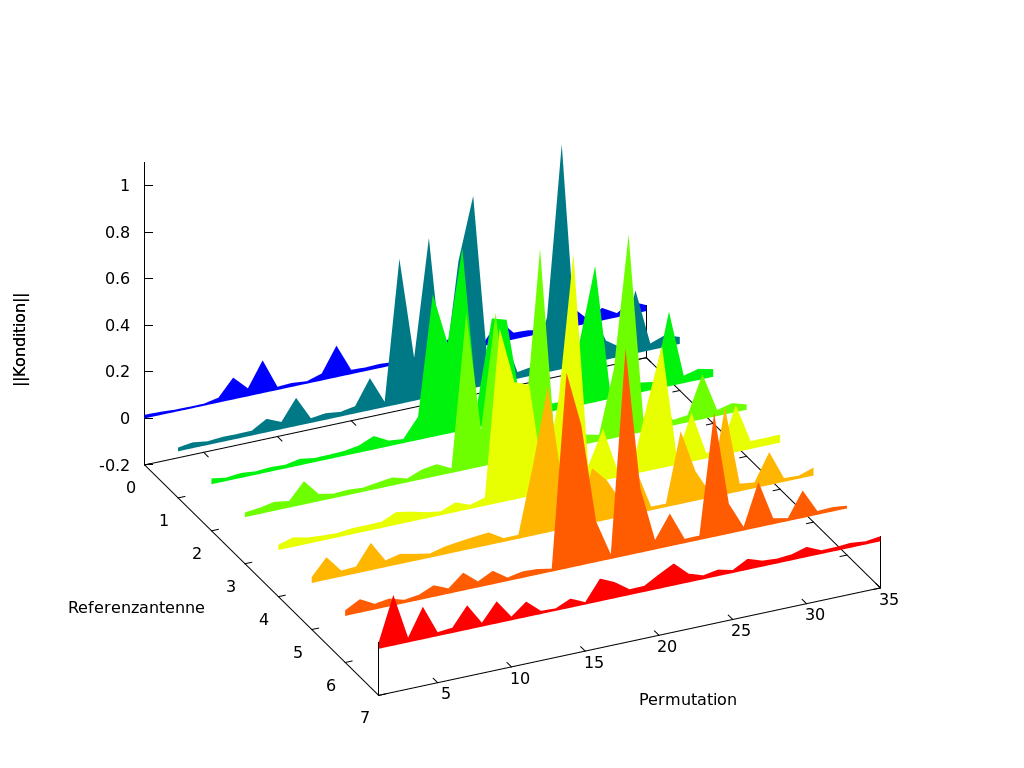
\includegraphics[width=\textwidth]{img/fenceModell9x3.png}
                 \caption{Konditionszahl der $10\times3$ Matrix normiert auf den größten vorkommenden Wert ($=257,13$); In dieser Konfiguration sind die Konstanten ($a_1$ \& $a_2$) sowie die variablen, gemessenen Phasen $\Theta_k$ enthalten}
                 \label{fig:AnalyzeOf10x3}
         \end{subfigure}
%
\end{figure}
%
Aus der Grafik lässt sich entnehmen, dass es für jede Referenzantenne aus der Geometrie alleine gute Konfigurationen existieren. Aus diesen Erkenntnissen kann in späteren Aufbauten, die Position der Antennen optimiert werden. Diese Verfahren wird in Abschnitt~\ref{sec:Calibration_Optimaztion} weiter beschrieben.
%
%- Section 2.3 --------------------------------------------------------------
\subsection{Weitere Anwendung der Konditionszahl}
Weitere Anwendungen, die sich aus der Konditionszahl der Matrix ableiten, sind denkbar. Für die FPGA-Software ist, parallel zu diesem Projekt, eine intelligente Umschaltung der Antennen in der Planung. Die Kondition der geometrische Matrix verändert sich nach dem Kalibrieren nicht mehr. Dadurch und durch die oben beschriebenen Überlegungen kann statisch eine Abschätzung für die Konditionszahl, von zwei der drei Blockmatrizen, im Vorfeld erstellt werden. Die Konditionszahl dient zum Steuern der Umschaltung. Ordner man die möglichen Konfiguration anhand ihrer Konditionszahl (niedrigste zuerst) in einer statischen Liste an so kann im FPGA eine einfache, schlaue Umschaltung implementiert werden. Diese würde immer dafür sorgen, dass Messdaten von einer Konfiguration bevorzugt werden, die eine niedrige Konditionszahl hat und somit relativ sicher zu einer guten Lösung führen. Diese überlegungen werden im Rahmen dieser Arbeit nicht näher beschrieben.\\
Eine Weitere Anwendung ergibt sich für die Kalibrierung. Der Aufbau der Antennen kann unter Berücksichtigung der Kondition optimieren. Ziel der Optimierung wäre es durch eine geeignete Positionierung der Antennen, die Anzahl der Antennenpermutationen mit kleiner Konditionszahl zu maximieren.
%
%---------------------------------------------------------------------
\section{Einsatz des Modells}
\label{sec:use_of_model}
Im vorherigen Abschnitt wurde das Modell aus den geometrischen Gegebenheiten hergeleitet. Das Modell ist in seinen Eingabeparametern Flexibel und erlaubt verschiedene Arten des Einsatzes. Diese werden im Folgenden erläutert.
%
\input{chapters/1_main/sections/use_of_model.tex}
%
%---------------------------------------------------------------------
\section{Realisierung der Kalibrierung}
\label{sec:calibration}
In diesem Abschnitt wird die Implementierung der Kalibrierung des Messaufbaus und kurz die Ergebnisse zusammengefasst. Es werden zwei unterschiedliche Berechnungsverfahren vorgestellt. Zuerst die Berechnung über das SVD-Verfahren, danach durch das CMA-ES-Verfahren. Es ist sinnvoll zu erwarten, dass beide Ergebnisse die gleichen Koordinaten liefern.
%
\subsection{Implementation}
%
Der Ablauf der Kalibrierung ist in Abbildung~\ref{fig:calibration_flowchart} in Form eine Ablaufdiagramms dargestellt. Beschrieben werden die wesentlichen Schritte. Es sind sowohl Interaktion mit der Person enthalten die die Kalibrierung durchführt, als auch die Schritte die von den beteiligten Softwarekomponenten ausgeführt werden enthalten. Es wurden im Rahmen der Arbeit zwei unterschiedliche Wege implementiert, ein Ergebnis für die Kalibrierung zu berechnen. Diese Wege werden nun kurz vorgestellt. Un die Ergebnisse mit einander verglichen. Die Präsentation der Resultate wird auch dazu verwendet werden die gewählte Form der Diagramme zu erläutern. Diese werden in den Ergebnissen des komplexeren Modells ebenfalls verwendet.
%
\begin{figure}[H]
	\begin{center}
		\caption[Ablauf der Kalibierung]{Ablauf der Kalibierung}
		\label{fig:calibration_flowchart}
		\vspace{0.5cm}
		\begin{tikzpicture}[auto]
		\scriptsize
			\tikzstyle{decision} = [diamond, draw=black, thick, fill=black!20, text width=5em, text badly centered, inner sep=1pt]
%			
			\tikzstyle{block} = [rectangle, draw=black, thick, fill=gray!20, text width=15em, text centered, rounded corners, minimum height=4em]
%	
			\tikzstyle{line} = [draw, thick, -latex',shorten >=1pt];
			\tikzstyle{commentline} = [draw, dashed, green!50,-latex',shorten >=1pt];
%	
			\tikzstyle{cloud} = [ dotted, draw=green!50, thick, ellipse,,fill=green!20, minimum height=2em, text width= 10em, text badly centered];
%	
			\matrix [column sep=5mm,row sep=7mm]
			{
				% row 1
				& \node [block] (start) { Start }; & \\
				% row 2
				& \node [block] (setup) {Aufstellen des Kalibrierstücks}; & 
					\node [cloud] (comment1) {Gezeigt in Abbildung \ref{fig:calib_piece}}; \\
				% row 4
				& \node [block] (measure) {Vermessen der Entfernungen zu den Antennen}; & 
					\node [cloud] (comment2) {z.B. mit Laser-Entfernungsmesser, gezeigt in Abbildung \ref{fig:laser_meter}}; \\
				% row 5
				&\node [block] (writefile) {Eintragen der Vermessenen Werte in Mashinenlesbare Datei}; &\\
				% row 6
				\node (temp){}; &\node [block] (startsw) {Starte die Kalibiersoftware}; &\\
				% row 7
				&\node [block] (viewresults) {Speichern der berechneten Werte}; &\\
				% row 8				
				& \node [decision] (decide) {$\Delta \geq \Delta_{max}$}; & 
					\node [cloud] (criteria) {Ergebnisse haben eine geringe Abweichung};\\
				% row 9
				& \node [block] (stop) {Ende}; & \\
			};
			
%
%			Draw the arrows
%
			\path (decide) -| node [near start] {Nein} (temp);
			\tikzstyle{every path}=[line]
			\path (start) -- (setup);
			\path (setup) -- (measure);
			\path (measure) -- (writefile);
			\path (writefile) -- (startsw);
			\path (startsw) -- (viewresults);
			\path (viewresults) -- (decide);
			\path (decide)	-| +(-3,0)  |- (measure);
			\path (decide) -- node [midway] {Ja} (stop);
			
%			
%			draw the comments 
%
			\tikzstyle{every path}=[commentline]
			\path (criteria) -- (decide);
			\path (comment1) -- (setup);
			\path (comment2) -- (measure);
				
		\end{tikzpicture}
	\end{center}
\end{figure}

\subsubsection{SVD}
%
Das unter \ref{sec:svd} vorgestellte Verfahren der Singular-Value-Decomposition kann dazu verwendet werden eine Lösung eines Gleichungssystems zu berechnen. Das Modell, dass zur Kalibrierung verwendet wird, ist ein Gleichungssystem der Form $\mathbf{b}=\mathbf{A}\mathbf{x}$ und hat drei Gleichungen mit drei Unbekannten. Daher kann sofort eine Lösung mit dem Verfahren hergeleitet werden. Das Ergebnis eines Messaufbaus mit 3 Antennen ist in Tabelle\ref{tab:FinalCoords} und in Abbildung~\ref{fig:3dplot_coordinates} gezeigt. Die Implementation des Algorithmus stammt aus \cite{press2007numerical} und wurde für diese Arbeit angeschafft.
%
\subsubsection{CMA-ES}
Das über den evolutionären Algorithmus gefundene Ergebnis gleicht dem des SVD-Verfahrens. Der SVD-Algorithmus ist um ein vielfaches effizienter beim Lösen des Gleichungssystems. Der Gründe warum an dieser Stelle das Ergebnis dennoch über evolutionäre Verfahren dargestellt wird sind folgende:
%
\begin{enumerate}
 \item Die Komplexität ist gering, daher kann der Ablauf des evolutionären Verfahrens besser dargestellt und verstanden werden
 \item Der Vergleich der beiden Ergebnisse ermöglicht die Verifizierung der Implementation beider Verfahren.
\end{enumerate}
%
Der erste Punkt kommt im Rahmen dieser Arbeit eine besondere Stellung zu, es ist einfacher anhand dieses Übersichtlichen Problems (mit nur drei Unbekannten) den Ablauf des Algorithmus sowie die Visualisierung der Ergebnisse besser zu erläutern. Die verwendete Darstellung gleicht der, die später bei dem Komplexeren Modell Verwendung findet.
%
\subsection{Ergebnis}
Es werden nun die Ergebnisse der Kalibrierung vorgestellt. Für eine der Vermessenen Antennenkonfigurationen sind in der folgenden Tabelle die Koordinaten der Antennen gezeigt. Die Visualisierung der Konfiguration zeigt die Abbildung~\ref{fig:3dplot_coordinates}.
%
\begin{table} [!ht]
	\begin{center}
		\begin{tabular}{cccc}
		      \textbf{Antenne} & \textbf{x} & \textbf{y} & \textbf{z} \\
		      1 &	0.479	&	-1.012 & 0.60 \\
		      2 &	-0.77 	&	-1.04 & 1.34 \\
		      3 &	1.52  	&	-1.05 & 1.37 \\
		      4 &	-0.92 	&	-0.19 & 1.32 \\
		      5 &	1.92 	&	0.03 & 1.39 \\
		      6 &	-0.55 	&	1.09 & 1.43 \\
		      7 &	1.06 	&	1.07 & 1.35 \\
		      8 &	0.45 	&	1.35 & 0.67 \\
%		      
		\end{tabular}
		\caption[Finale Antennen Koordinaten]{Tabelle der finalen Antennenkoordinaten [m], berechnet mit dem in dieser Arbeit entwickelten Modell und dem SVD-Verfahren, die Ergebnisse wurden auf zwei Nachkommastellen gerundet und sind identisch für beide Methoden.}
		\label{tab:FinalCoords}
	\end{center}
\end{table}
%
Eine Berechnung mit dem evolutionären Verfahren dauerte ca. $170~ms$ mit dem SVD-verfahren wurde eine Lösung und $\le 1~ms$ gefunden. Für die in der Praxis eingesetzte Software wird es eine Implementation der Kalibrierung mit dem SVD-Verfahren geben. Das Ergebnis der mit dieser Variante berechnete Verfahren wird bei Bedarf mit einer Lösung des evolutionären Verfahrens verglichen. Das ermöglicht eine Build-In Verifikation der Kalibrierung.\\

Für die in den folgenden Abbildungen präsentierten Ergebnisse wurden insgesamt $100$ Durchläufe des Algorithmus erstellt. Die Ergebnisse wurden mit einem vom Algorithmus selbst erstellten $\mu$ und $\lambda$ gefunden. In Abbildung~\ref{fig:Final_Calibration_Ant0_ES-boxes} wird eine statistische Auswertung der Ergebnisse gezeigt. In jedem Plot werden die Endwerte der Lösungen in einem sog. Boxplot gezeigt. Dabei wird die Verteilung mit Hilfe von Boxen dargestellt. Die Fähnchen der Boxen, stellen die maximal- bzw. minimal-Werte dar. Die Größe der Boxen enthält das obere und untere Quartil der Daten, der horizontale Strich in der Box zeigt den Mittelwert der Daten. Ausreißer in den Daten werden durch Punkte abseits der Box dargestellt.\\
%

Die Abbildung.~\ref{fig:Final_Calibration_Ant0_ES-boxes} zeigt den Verlauf der drei Objektvariablen (x,y,z-Koordinaten) sowie die Entwicklung der Fitness und des mittleren Sigmas. Als Darstellungsart wird der Linienplot verwendet und überlagern die Verläufe der einzelnen Lösungen. Das Abbruchkriterium war eine Fitness von $\leq 10^{-25}$. Für Darstellungszwecke wurde die x-Achse nach $500$ Werten beschränkt, erreicht der Fitness-Plot diesen Wert in der Abbildung nicht. Der Verlauf ist typisch für den Verwendeten Algorithmus. Deutlich zu erkennen ist eine Verbesserung des Ergebnisses mit steigender Zahl der Generationen. Der Verlauf der Variablen ist immer für den Erfolgreichsten Nachkommen einer Generation dargestellt.\\
%

Abbildung~\ref{fig:Final_Calibration_Ant0_ES-Scatter} ist ein Scatter-Plot. Die Objektvariablen werden hier gegeneinander aufgetragen. Auf der Diagonalen befinden sich stets die Variable mich sich selbst, daher zeigt sich dort eine Linie bzw. ein einzelner Punkt, sollten die Ergebnisse nicht streuen. Der Plot ist praktisch um die Implementation des Algorithmus zu verifizieren. Er lässt Rückschlüsse auf Abhängigkeiten und Einflüsse der Objektvariablen zu. So können die Ergebnisse mit den Erwartungen verglichen werden.\\
%
%---------------------------------------------------------------
%
\begin{figure}[!ht]
  \begin{center}
    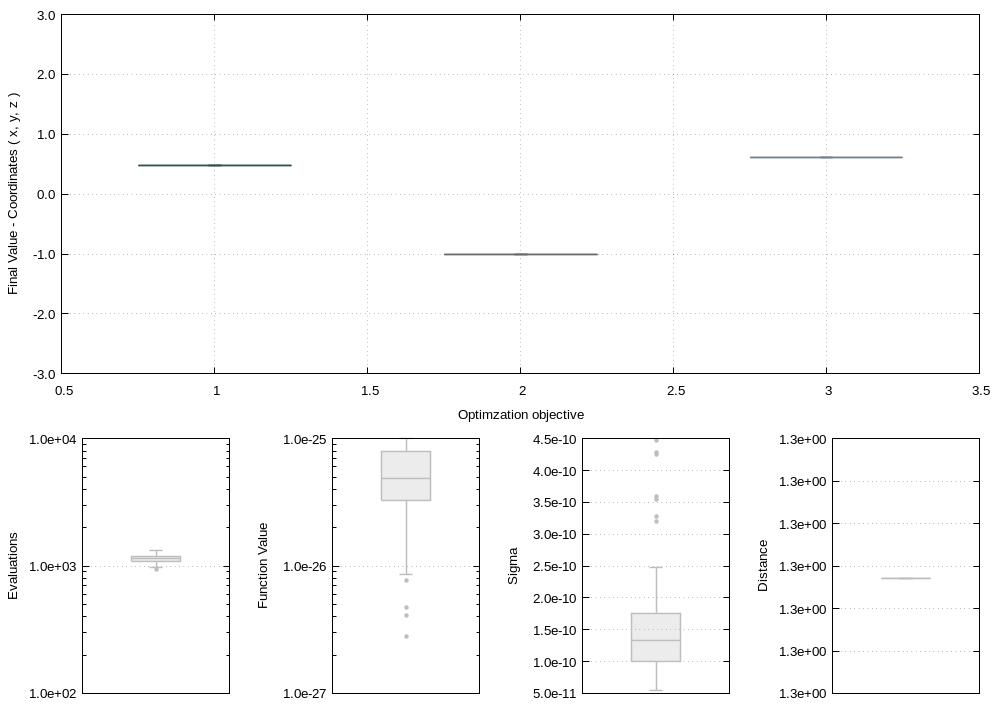
\includegraphics[width=0.9\textwidth]{img/calibration/calibration_ant0-boxes.png}
  \end{center}
  \caption {Boxplot des Kalibierergebnis aus $100$ Durchläufen. Im oberen Plot der sind die x,y,z-Koordinaten gezeigt, diese landen in allen Durchläufen auf dem selben Ergebnis. Das zeigt sich in der Breite der Linien. Die unteren vier Plots zeigen die Anzahl der Evaluationen der Fitness-Funktion, den finalen Funktionswert, das Sigma für die Variablen, die Entfernung zum Referenzpunkt (v.l.n.r.).}
  \label{fig:Final_Calibration_Ant0_ES-boxes}
%
\end{figure}
%
%---------------------------------------------------------------
%
\begin{figure}[!ht]
  \begin{center}
    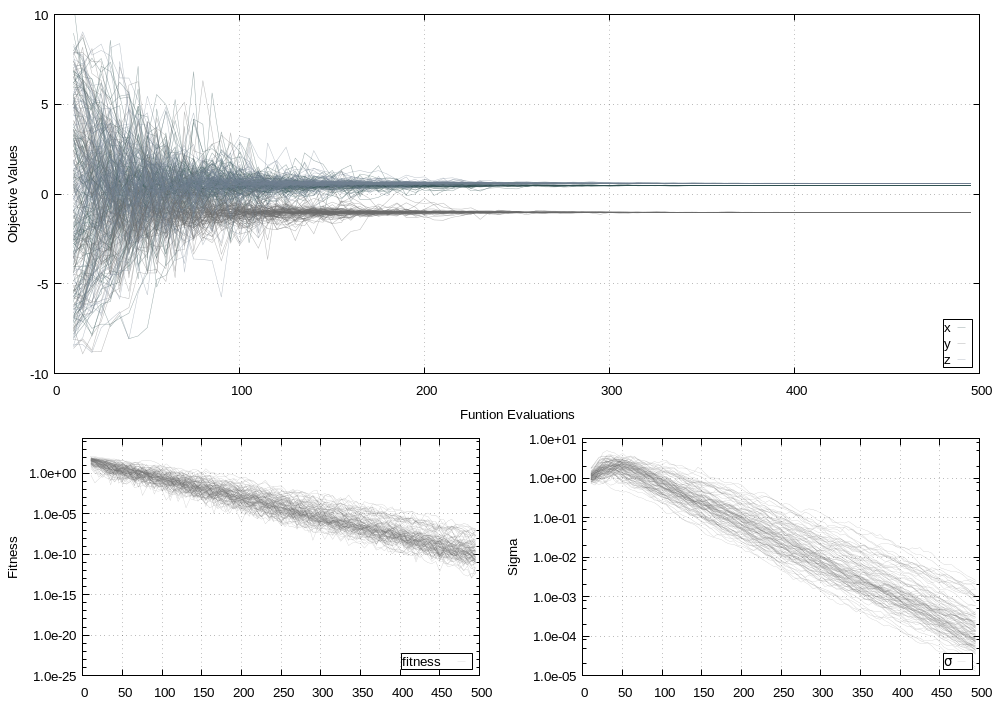
\includegraphics[width=0.9\textwidth]{img/calibration/calibration_ant0-lines.png}
  \end{center}
  \caption {Zu erkennen ist, das nach ca. 300 Evaluationen der Zielfunktion keine großen Änderungen der Variablen zu erkennen sind. Bis zum erreichen des Abbruchkriteriums (Function Value $\leq10^{-25}$) werden noch ca 400 Evaluationen benötigt, vgl. korrespondierender Boxplot.}
  \label{fig:Final_Calibration_Ant0_ES-Lines}  
%  
\end{figure}
%---------------------------------------------------------------
%
\begin{figure}[!ht]
  \begin{center}
    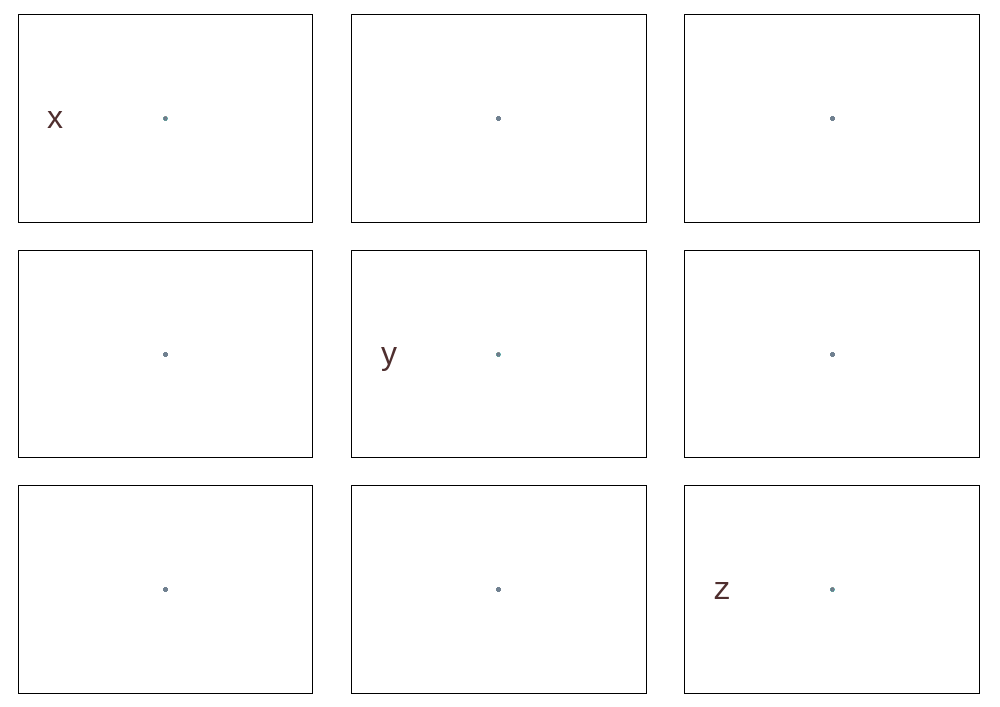
\includegraphics[width=0.9\textwidth]{img/calibration/calibration_ant0-scatter.png}
  \end{center}
  \caption {Scatter-Plot der Ergebnisse der evolutionären Kalibrierung. Die Endergebnisse streuen in keiner Dimension, das wird aus dieser Darstellung deutlich.}
  \label{fig:Final_Calibration_Ant0_ES-Scatter}  
%  
\end{figure}
%---------------------------------------------------------------
%
\lipsum[1]
%
\begin{figure}[!ht]
         \centering
         \begin{subfigure}[h]{0.4\textwidth}
                 \centering
                 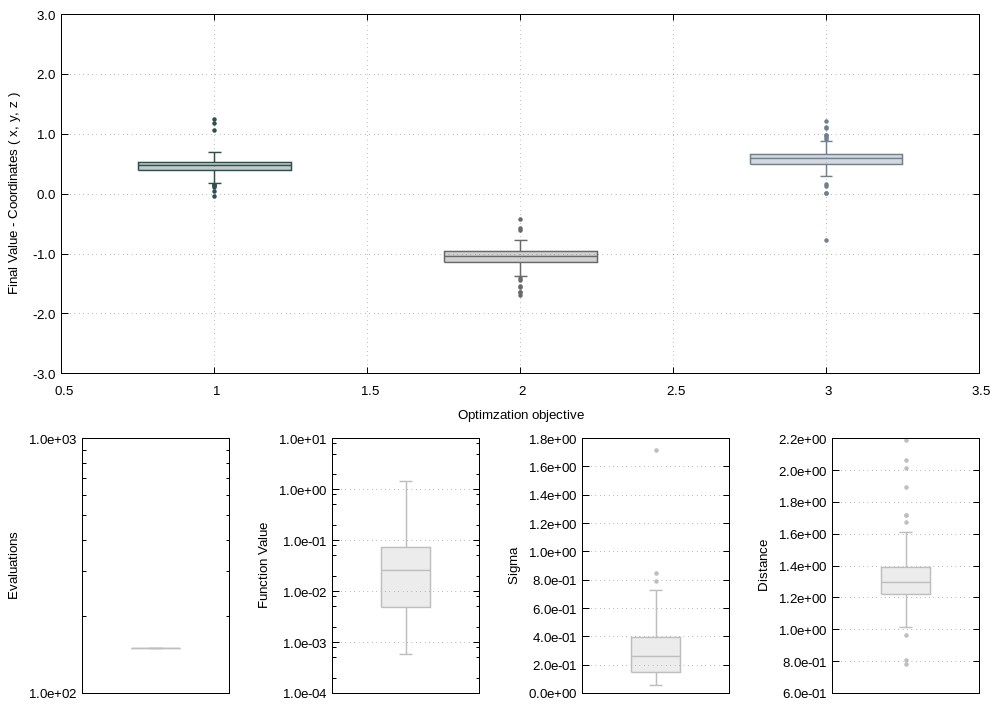
\includegraphics[width=\textwidth]{img/calibration/aborted_calibration_ant0-boxes.png}
                 \caption{Statistisch verteilte Endwerte für die Koordinaten der Kalibrierung. Die Werte für x,y, und z haben noch nicht ihren Endwert erreicht.}
                 \label{fig:abortedFinal_Calibration_Ant0_ES-boxes}
         \end{subfigure}
%
\qquad         
%
         \begin{subfigure}[h]{0.4\textwidth}
                 \centering
                 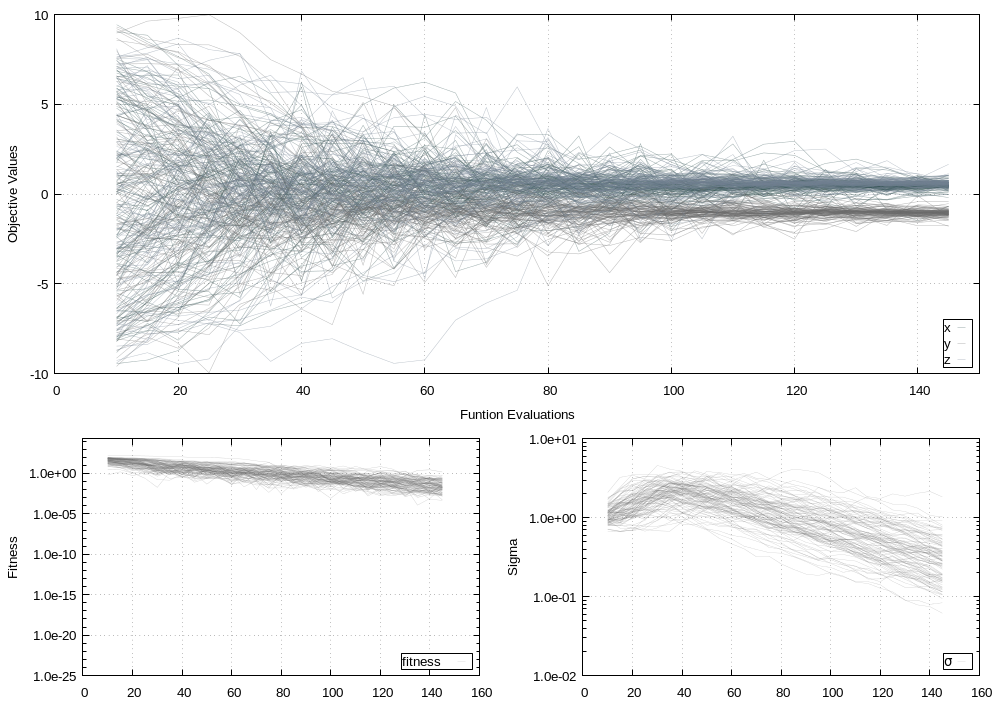
\includegraphics[width=\textwidth]{img/calibration/aborted_calibration_ant0-lines.png}
                 \caption{lorem}
                 \label{fig:abortedFinal_Calibration_Ant0_ES-Lines}
         \end{subfigure}
%
\\
%
         \begin{subfigure}[h]{0.4\textwidth}
                 \centering
                 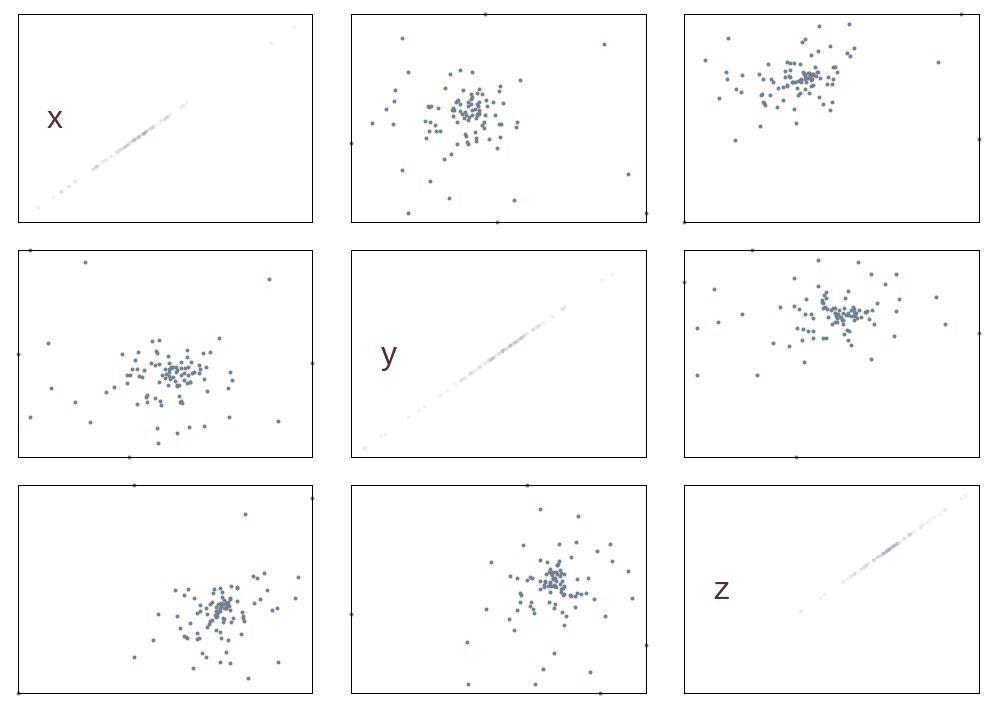
\includegraphics[width=\textwidth]{img/calibration/aborted_calibration_ant0-scatter.png}
                 \caption{lorem}
                 \label{fig:abortedFinal_Calibration_Ant0_ES-Scatter}
         \end{subfigure}
%
         \caption[Statistisch verteilte Ergebnisse der Evolutionären Kalibrierung]{Analog zu der Abbildung \ref{fig::Final_Calibration_Ant0} zeigen die Plots die gleichen Darstellungen. Diese zeigt, wie sich eine Statistische Verteilung in den Plots Manifestieren würde. Um das zu demonstrieren wurde das Abbruchkriterium auf lediglich $150$ Evaluationen der Zielfunktion eingestellt. Zu diesem Zeitpunkt können die Objektvariablen bereits einen passablen Wert erreicht haben oder noch abweichende Werte aufweisen (vgl. \ref{fig:Final_Calibration_Ant0_ES-Lines}).}
         \label{fig::abortedFinal_Calibration_Ant0_ES}
\end{figure}
%
\begin{figure}[ht!]
         \centering
         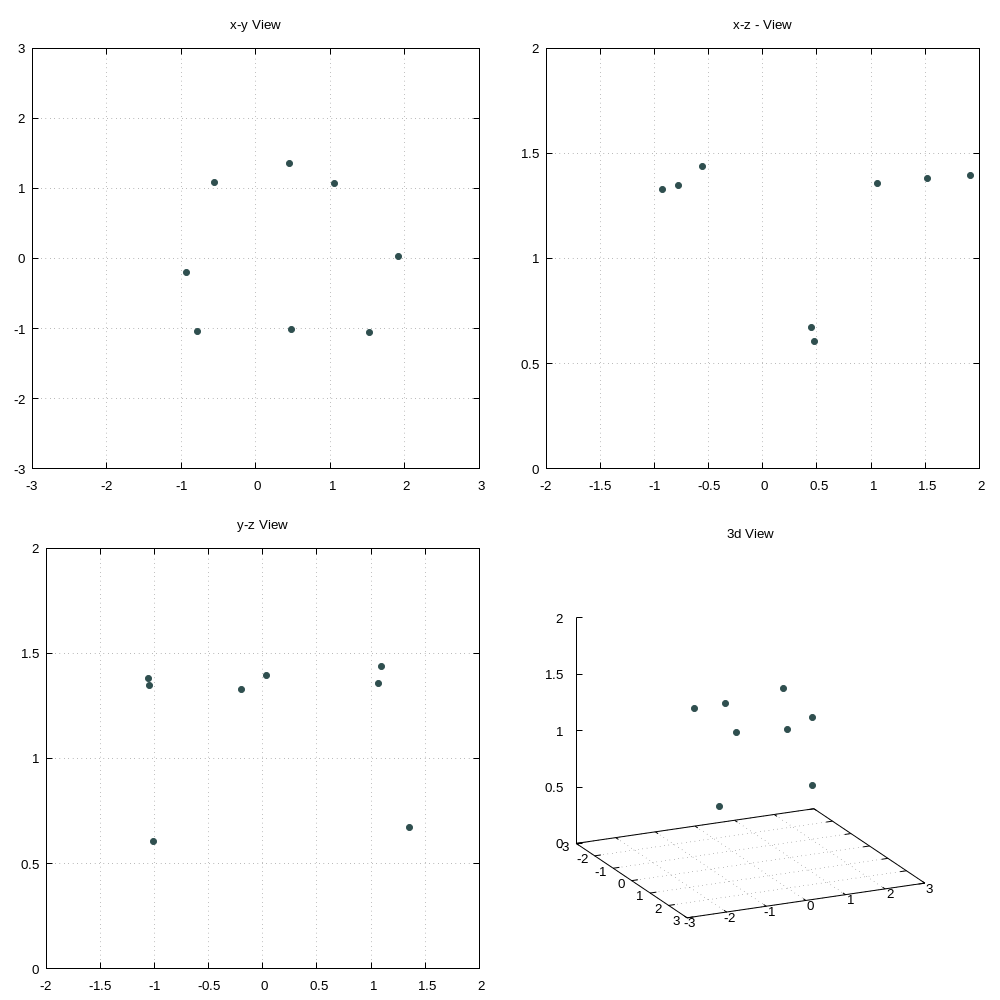
\includegraphics[width=0.7\textwidth]{img/calibration/calibration_results.png}
         \caption[Visualisierung des Kalibrierendergebnis]{Visualisierung des Kalibrierendergebnis. Abgebildet sind die gefundenen Antennenkoordinaten (Punkte) in drei Raumansichten. Die zusätzliche, dreidimensionale  Ansicht dient der Überischt.}
         \label{fig:3dplot_coordinates}
%
\end{figure}
%
\begin{figure}[ht!]
         \centering
         \caption[Kalibrierwerkzeuge]{Werkzeuge die bei der Kalibrierung verwendet werden.}
         \begin{subfigure}[h]{0.4\textwidth}
                 \centering
                 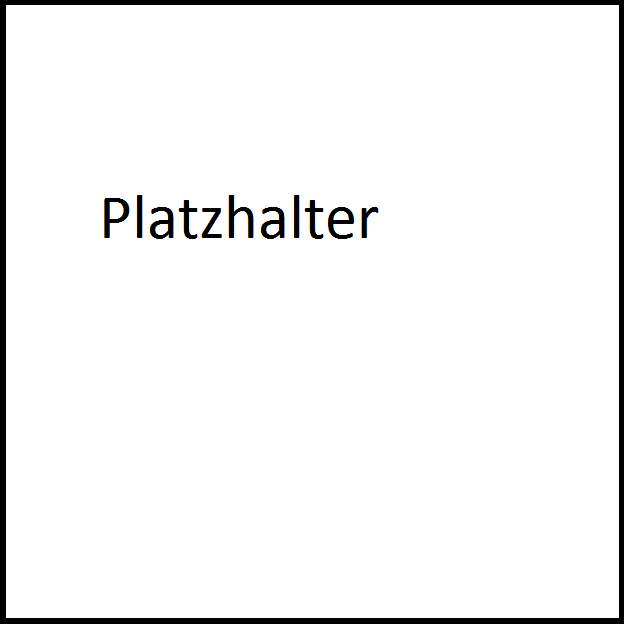
\includegraphics[width=\textwidth]{img/00_placeholder-sqare.png}
                 \caption{Laser Distanzmesser}
                 \label{fig:laser_meter}
         \end{subfigure}
%
\qquad         
%
         \begin{subfigure}[h]{0.4\textwidth}
                 \centering
                 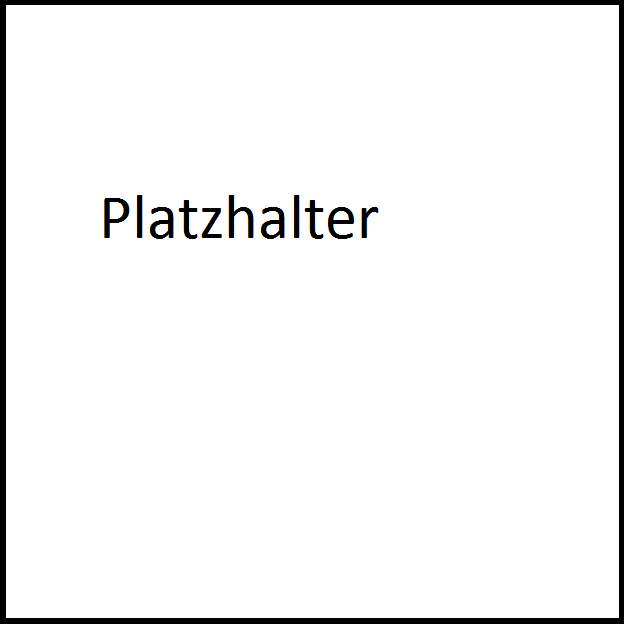
\includegraphics[width=\textwidth]{img/00_placeholder-sqare.png}
                 \caption{Kalibrierstück}
                 \label{fig:calib_piece}
         \end{subfigure}
         \label{fig:Calibration_Tools}
\end{figure}
 
%
%---------------------------------------------------------------------
\section{Betrachtung der Komplexität}
\label{sec:Komplexity2}
%
Im Folgenden wird eine Betrachtung der Komplexität des in Abschnitt~\ref{sec:model_developement} entwickelten Modells präsentiert. Diese Betrachtung ist wichtig für die Parametrisierung des Optimierungsverfahrens sowie für eine Beurteilung der Generellen Lösbarkeit mit den verwendeten Verfahren. Es wird eine Visualisierung des Fitness-Raums vorgestellt und im Vergleich mit sog. Benchmark-Funktionen diskutiert.\\
%

Für die Erstellung der Fitness-Ebenen wurde ein Programmteil (der \textit{FitnessPlaneCalculator}) entwickelt, der ein Modell mit vorgegebenen Daten füttert und den Rückgabewert in eine Datei schreibt. Das Programm lässt sich per Eingabedatei steuern und erlaubt die Definition der Ebenen die dargestellt werden sollen. Es lassen sich immer zwei Variablen der Objektfunktion variieren und der Rest wird dabei auf feste Werte gesetzt. Das erlaubt eine Visualisierung durch eine 2D-Heatmap (siehe folgende Plots). Aus der Visualisierung können Rückschlüsse auf die Gestalt der Fitnessebene gezogen werden.\\
%

Die Parameter wurde für diese Plots so gewählt das sie über einen Bereich iterieren, indem die richtige Lösung liegen sollten. Da nur drei Parameter variiert werden, werden die übrigen vier auf analytisch bestimmte, wahre Werte gesetzt. Diese sind in Tabelle~\ref{tab:complexity1} zusammen mit den wahren Werten aufgeführt.\\

%
\begin{figure}[h!]
  \caption[Fitness Ebenen Heatmap]{Diese Grafik zeigt die Fitnessebenen des Problems für eine Anordnung aus vier Antennen und einem Sweep über die $x-y$ - Ebene. Jeder Plot ist für einen festen Wert $z$ erstellt worden. In der Oberen linken Ecke beginnend und nach rechts laufend. Die $x, y$-Werte wurden über ein Intervall von $[-5,5]$ m und mit einem Inkrement von $0.2$ variiert. Daraus ergibt eine für die Abschätzung der Gestalt der Fitnessebene ausreichende Datengrundlage. Die $z$-Werte der $16$-Plots stammen aus dem Intervall $[-7,-7]$ mit einem Inkrement von $1$. Bereits in dieser Ansicht, ist zu erkennen, dass der Verlauf sehr Flach ist. Eine Schlucht bildet sich etwa in Nord-Süd-Richtung aus. Jeweils verzeichnet ist das lokale Minima ($+$) eins Plots, sowie die Höhenlinien\footnote{Die Höhenlinien sind für diskrete Werte ${0,1,10,40,50,100,200,500,1000}$ erstellt worden}. Die farbliche Kodierung gibt den Fitnesswert an diesem Punkt an. Die Fitnesswerte wurden normiert und um den Wert ihres Minimums verschoben.}
  \begin{center}
    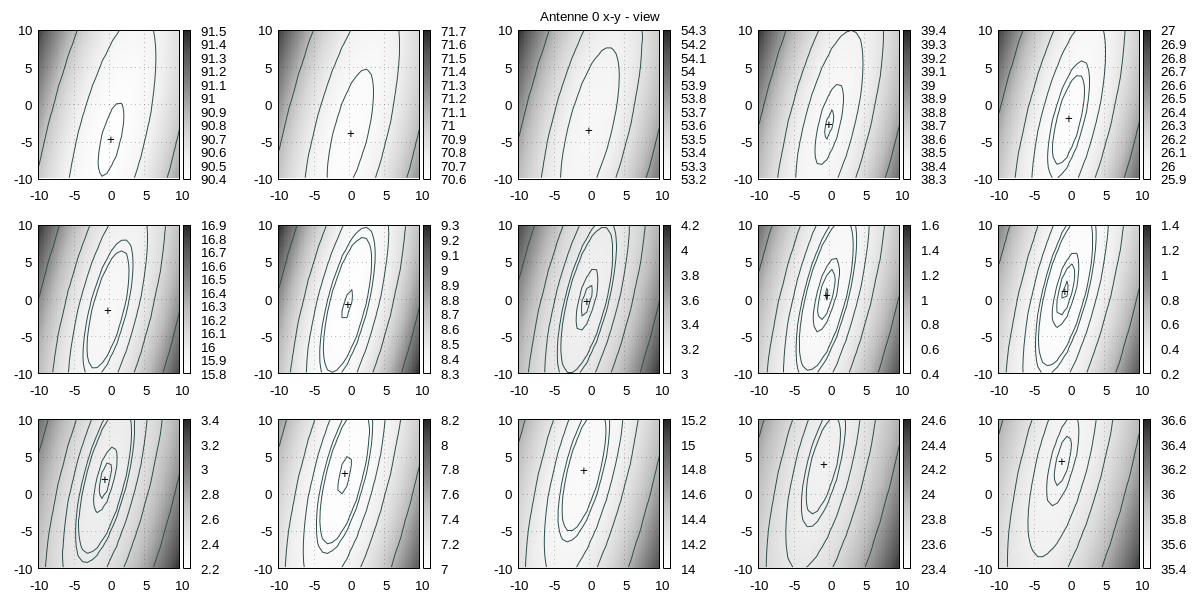
\includegraphics[width=\textwidth]{img/fitness/xy_a0.png}
  \end{center}
  \label{fig:fitnessplane1-x-y-1}
%
\end{figure}

\begin{figure}[ht!]
  \caption[Fitness Ebenen Heatmap, vergrößert]{Vergrößerung der Fitnessebenen der Antenne 1. Es ist hier deutlich zu erkennen, wie gering die Funktionen ansteigen. Das ist ein Problem für die meisten Algorithmen. Es bleibt zu klären wie sensitiv der Algorithmus auf diesen Umstand reagiert. Es wurde um das lokale Minima zentriert und der Bereich auf}
  \begin{center}
   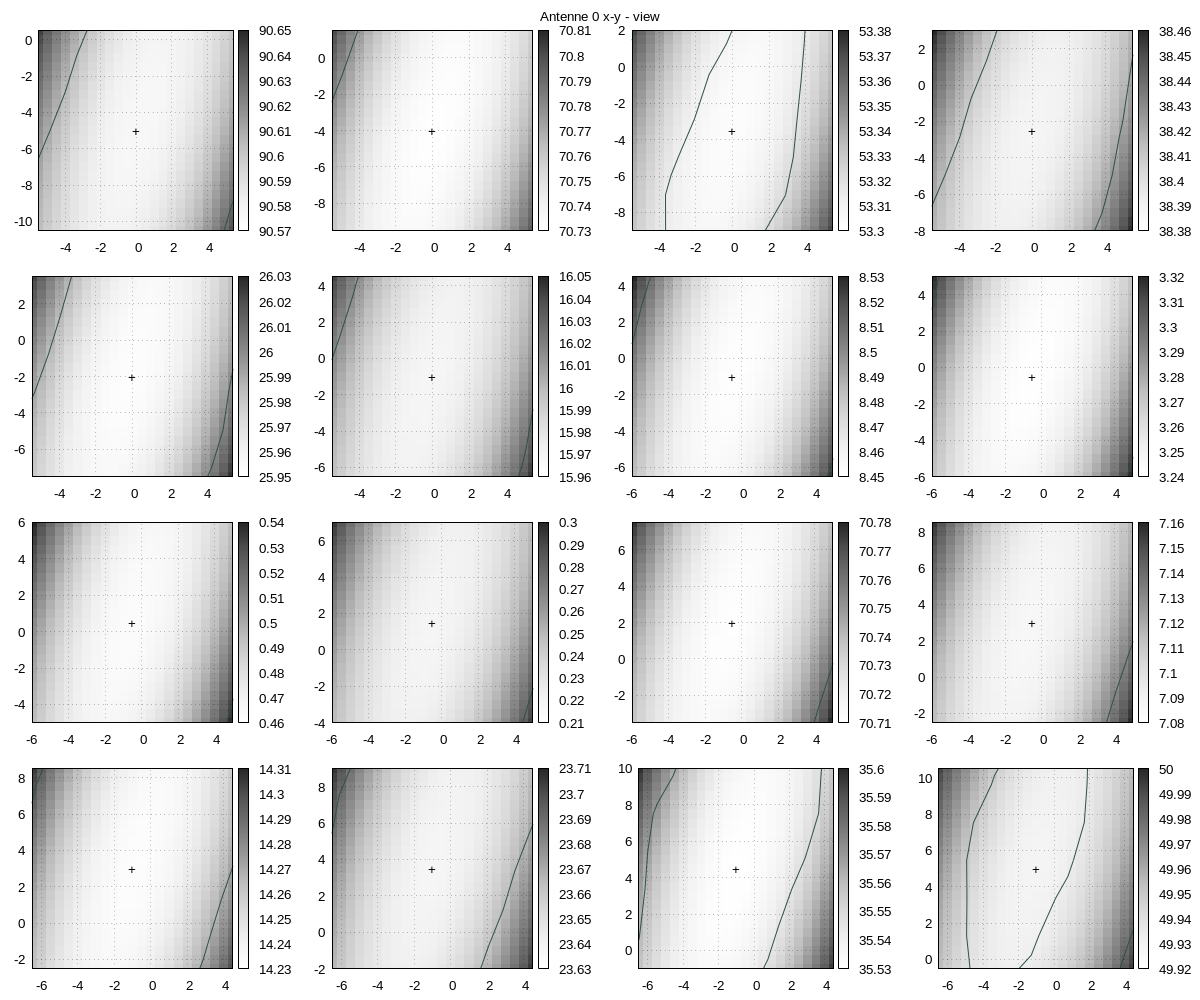
\includegraphics[width=\textwidth]{img/fitness/xy_a0zoomed.png}
  \end{center}
  \label{fig:fitnessplane1-x-y-zoom-1}
%
\end{figure}
%
In den Abbildungen~\ref{fig:fitnessplane1-x-y-1} und \ref{fig:fitnessplane1-x-y-zoom-1} zeigen sich möglicherweise die ersten Probleme für den Algorithmus. Eine große, sehr flache Fitnessebene für verschiedene Parameter ist nicht leicht zu handhaben. Aus dieser Untersuchung geht bereits hervor, dass die Anzahl an Nachkommen groß sein muss. Auch darf die Schrittweite $\sigma$ nicht zu klein werden, damit die Lösung nicht auf der flachen Ebene liegen bleibt. Ein Ähliches Verhalten zeigt sich bei den anderen Antennen und anderen Ebenen. Aufgrund der Komplexität des in dieser Arbeit erstellten Modells \ref{fig:Complexity1} ist bereits dieser Fall recht hochdimensional. Er erreicht $7$ Dimensionen und er kann im Rahmen dieser Arbeit nicht vollständig Untersucht werden. Die Fitness-Plots aller Antennen und für drei Ebenen sind in Anhang~\ref{app:fitness:plots1} zu finden. Eine vollständige Untersuchung ist indes auch nicht notwendig, da der Algorithmus den Suchraum in gewisser Weise untersucht. 
%
\begin{figure}[!h]
	 \caption[Übrige Ebenen für Antenne 1]{Auf diesen Abbildungen zeigen sich die Fitness-Ebenen für die übrigen Ansichten, x-z und y-z. In der oberen Reihe sind Ebenen über den gesamten Bereich, in der Unteren vergrößert dargestellt. Zu erkennen ist ein zum Verlauf der x-y-Ebene sehr ähnliches Bild. Ein flaches, längliches Tal mit Minimum.  }
	 \label{fig:fitnessplanesA1}
     \centering
     \begin{subfigure}[t]{0.4\textwidth}
             \centering
             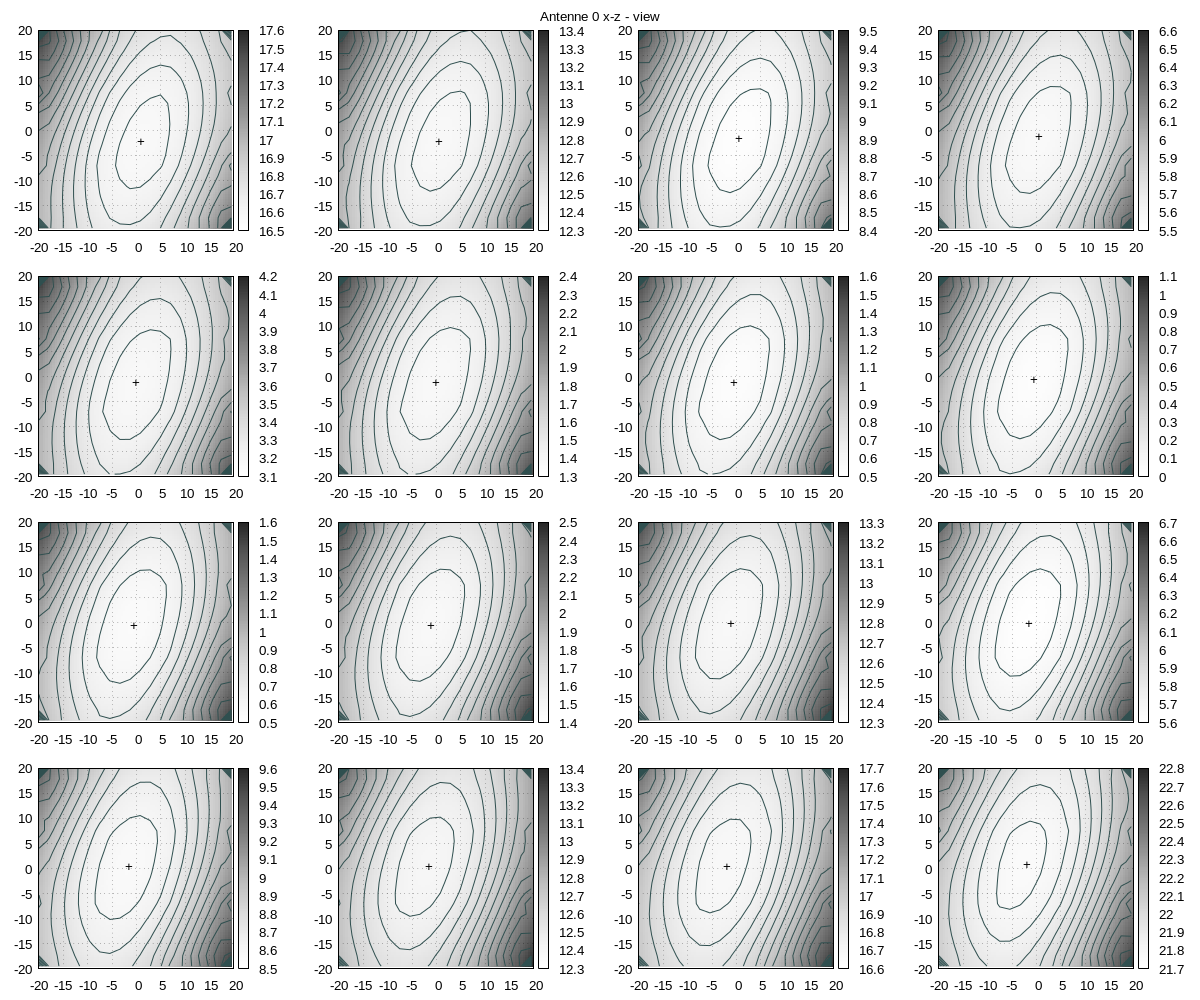
\includegraphics[width=\textwidth]{img/fitness/xz_a0.png}
%             \caption{Statistisch verteilte Endwerte für die Koordinaten der Kalibrierung.}
%             \label{fig:abortedFinal_Calibration_Ant0_ES-boxes}
     \end{subfigure}
     \qquad
     \begin{subfigure}[t]{0.4\textwidth}
			\centering
			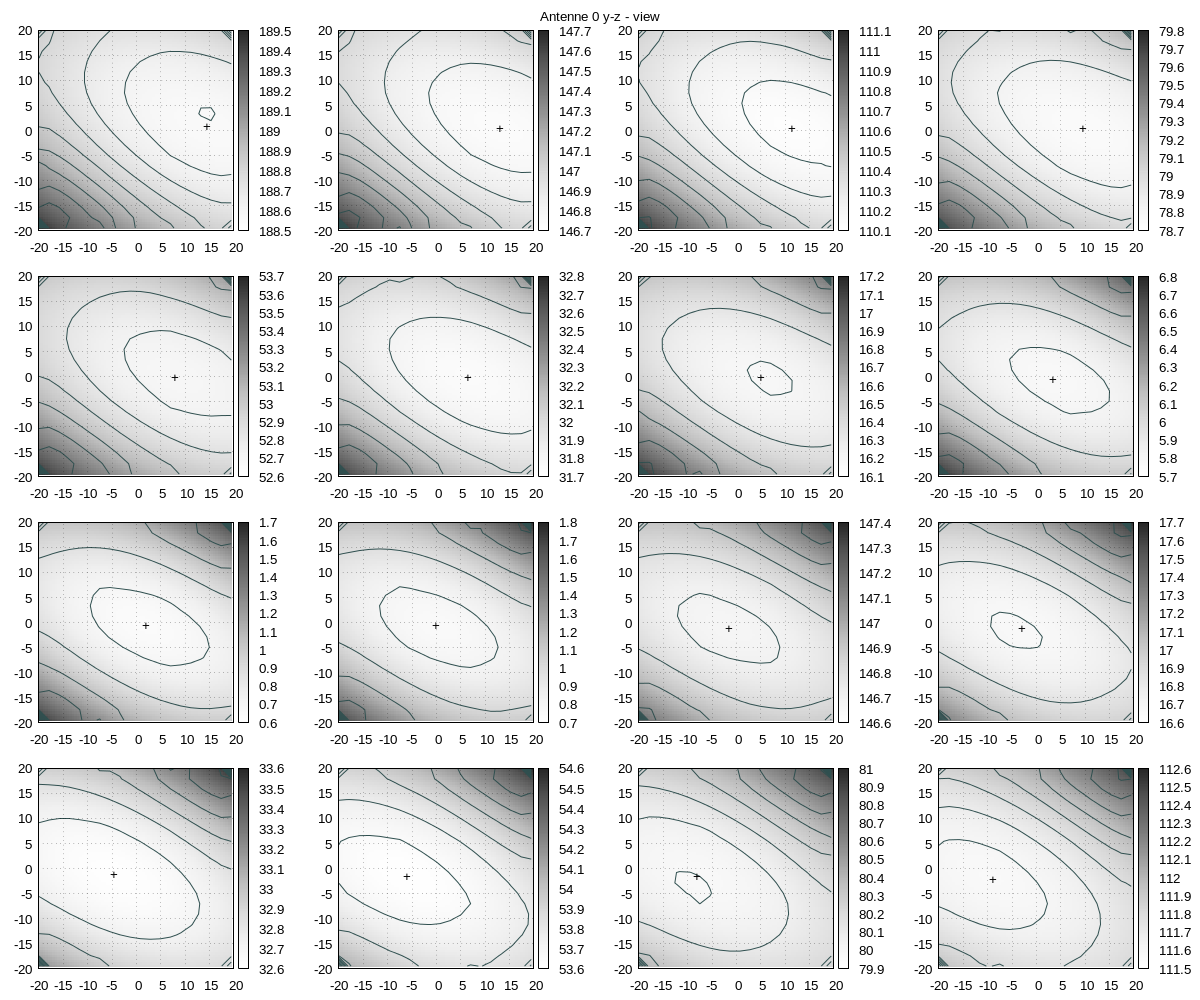
\includegraphics[width=\textwidth]{img/fitness/yz_a0.png}
%			\caption{x-z-Ebene, vergrößert}
%			\label{fig:abortedFinal_Calibration_Ant0_ES-boxes}
	 \end{subfigure}
\\
\vspace{5mm}
     \begin{subfigure}[t]{0.4\textwidth}
			\centering
			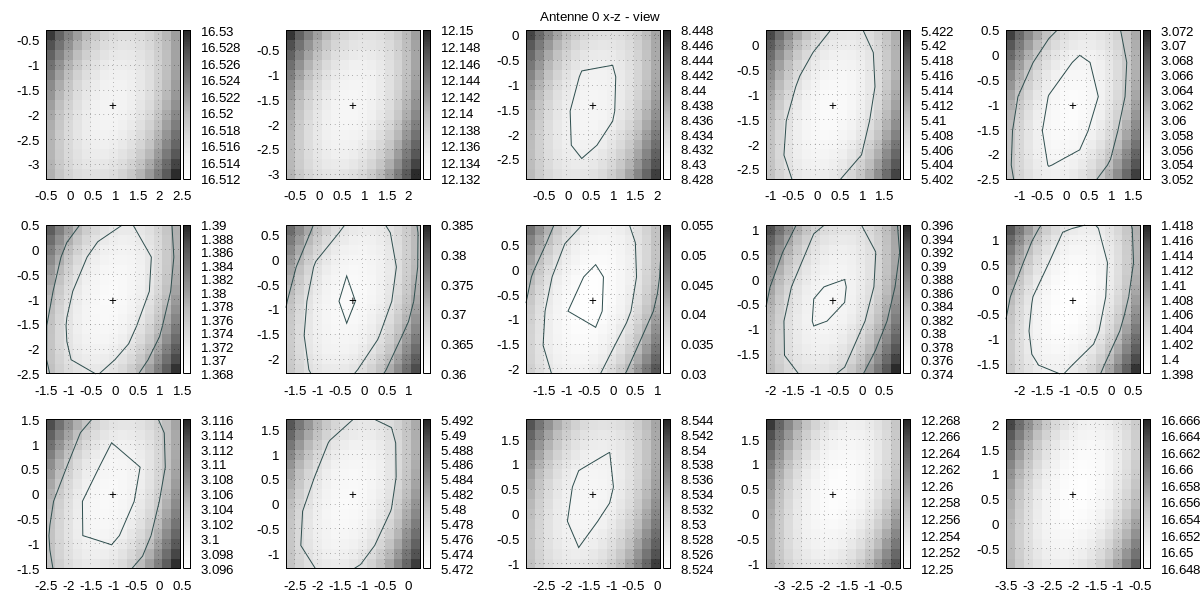
\includegraphics[width=\textwidth]{img/fitness/xz_a0zoomed.png}
%			\caption{x-z-Ebene, vergrößert}
%			\label{fig:abortedFinal_Calibration_Ant0_ES-boxes}
	 \end{subfigure}
	 \qquad
     \begin{subfigure}[t]{0.4\textwidth}
			\centering
			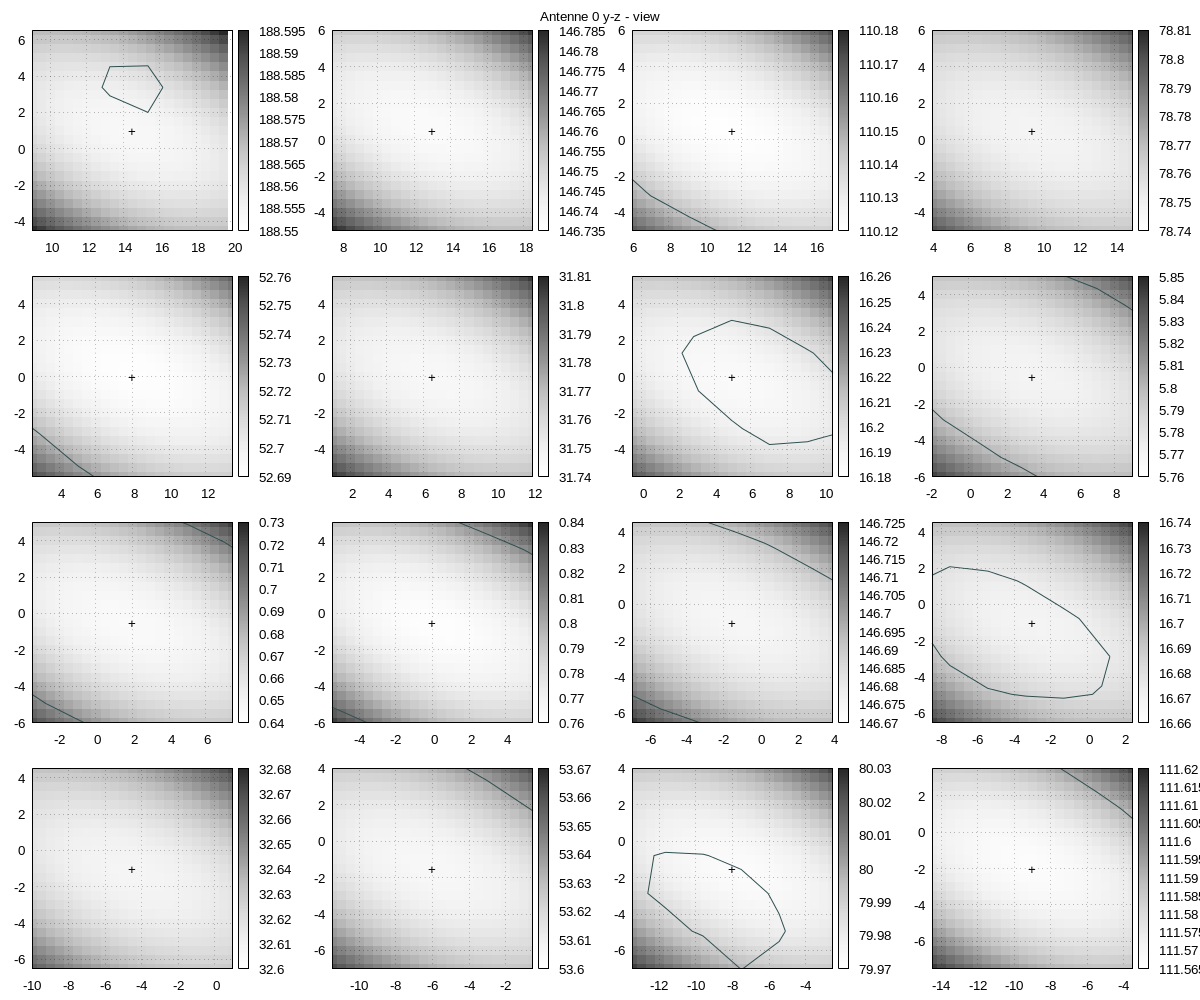
\includegraphics[width=\textwidth]{img/fitness/yz_a0zoomed.png}
%			\caption{x-z-Ebene, vergrößert}
%			\label{fig:abortedFinal_Calibration_Ant0_ES-boxes}
	 \end{subfigure}      
\end{figure}
%
\begin{table} [h]
	\begin{center}
		\begin{tabular}{lccccccc}
		\textbf{Ebene} & \textbf{$x$} & \textbf{$y$} & \textbf{$z$} & \textbf{$n_0$} & \textbf{$n_1$}& \textbf{$n_2$} & \textbf{$n_3$} \\
			\hline
			x-y & [-20:.5:20]		& [-20:.5:20]	& [-7:1:8] & [7:0:7] & [10:0:10]& [13:0:13]&[9:0:9]   \\
			x-z & [-20:.5:20] 	& [-7:1:8] 	& [-20:.5:20] & [7:0:7] & [10:0:10]& [13:0:13]&[9:0:9] \\
			y-z & [-7:1:8]  	& [-20:.5:20]	& [-20:.5:20] & [7:0:7] & [10:0:10]& [13:0:13]&[9:0:9]\\
			\hline
			Wahre & 0.479 & -1.012 & 0.607 & 7  & 10 & 13 & 9			\\
%
		\end{tabular}
		\caption[Parameter der Fitness Ebenen]{Tabellarisch sind hier die Parameter (Intervalle) der Fitness Ebenen aufgelistet. Zusätzlich sind die Werte angegeben, in denen eine optimale Lösung liegen sollte. }
		\label{tab:complexity1}
	\end{center}
\end{table}
%
%---------------------------------------------------------------------
\section{Software}
\label{sec:sw}
%
\lstset{
	basicstyle=\scriptsize,
	language=C++,
	breaklines=true,
	%		frameround=fttt,
	frame=tbrl,
	breakatwhitespace=false
	breaklines=true,  
	xleftmargin=1cm,
	tabsize=2,
	showstringspaces=false}
%---------------------------------------------------------------------
%
\subsection{Shark}
\label{sec:Shark}
Shark ist eine Open-Source \cpp Library für Maschinelles Lernen und Optimierung ~\cite{Shark:1}. Es Implementiert Methoden für lineare und nicht lineare Optimierung, Kernel-basierte Lernverfahren, künstliche neuronale Netzwerke, und Weitere. Details der Umsetzung finden sich in~\cite{shark08}. Es wird sowohl in Forschung als auch industriellem Umfeld eingesetzt und implementiert, nach eigenen Angaben, Algorithmen die in anderen Libraries nicht verfügbar sind. Shark baut auf den \textit{Boost C++ Libraries} auf und verwendet CMake\footnote{CMake (cross-platform make) ist ein plattformunabhängiges Programmierwerkzeug für die Entwicklung und Erstellung von Software.}. Dadurch ist es nahezu auf jeder Plattform verfügbar. Die Integration in ein Projekt ist sehr einfach und daher wird es in dieser Arbeit eingesetzt.\\

Eine Integration von Shark in dem Software Ökosystem ist aufgrund der vielen Features sehr sinnvoll. Weitere Entwicklungen können vom Funktionsumfang partizipieren.

%
%---------------------------------------------------------------------
\subsection{Implementation}
\label{sec:Implementation}
In diesem Abschnitt wird auf interessante Details der Softwareimplementation eingegangen. Es ist nicht möglich im vollen Umfang die Implementation der Softare besprechen, dafür ist die Software zu Umfangreich\footnote{Für diese Arbeit wurden ca. $5000$ Zeilen Quellcode erstellt - einzelne Modelle nicht mitgerechnet}. Lediglich sollen hier die Implementationen verschiedener Evolutionsalgorithmen unter Verwendung von Shark gezeigt werden. Verschiedene Algorithmen wurden in Kapitel~\ref{sec:es-common} Es wird beispielhaft die Implementation einer Objektfunktion beschrieben, wie sie typischerweise in Shark vorgenommen wird.
%
%\begin{figure}[ht!]
	\begin{center}
		\caption[Integration PRPS Software]{Übersicht über die Integration des PRPS Evolution Moduls in die bestehende PRPS-Software}
		\label{fig:Integration-prpsevolutions}
		\vspace{1cm}
		\begin{tikzpicture}[auto]
		\scriptsize
			\tikzstyle{decision} = [diamond, draw=black, thick, fill=black!20, text width=5em, text badly centered, inner sep=1pt]
%			
			\tikzstyle{block} = [rectangle, draw=black, thick, fill=gray!20, text width=15em, text centered, rounded corners, minimum height=4em]
%	
			\tikzstyle{line} = [draw, thick, -latex',shorten >=1pt];
			\tikzstyle{commentline} = [draw, dashed, green!50,-latex',shorten >=1pt];
%	
			\tikzstyle{cloud} = [ dotted, draw=green!50, thick, ellipse,,fill=green!20, minimum height=2em, text width= 10em, text badly centered];
%	
			\matrix [column sep=5mm,row sep=7mm]
			{
				% row 1
				& \node [block] (start) { Start }; & \\
				% row 2
				& \node [block] (setup) {Aufstellen des Kalibrierstücks}; & 
					\node [cloud] (comment1) {Gezeigt in Abbildung \ref{fig:calib_piece}}; \\
				% row 4
				& \node [block] (measure) {Vermessen der Entfernungen zu den Antennen}; & 
					\node [cloud] (comment2) {z.B. mit Laser-Entfernungsmesser, gezeigt in Abbildung \ref{fig:laser_meter}}; \\
				% row 5
				&\node [block] (writefile) {Eintragen der Vermessenen Werte in Maschinenlesbare Datei}; &\\
				% row 6
				\node (temp){}; &\node [block] (startsw) {Starte die Kalibiersoftware}; &\\
				% row 7
				&\node [block] (viewresults) {Speichern der berechneten Werte}; &\\
				% row 8				
				& \node [decision] (decide) {$\Delta \geq \Delta_{max}$}; & 
					\node [cloud] (criteria) {Ergebnisse haben eine geringe Abweichung};\\
				% row 9
				& \node [block] (stop) {Ende}; & \\
			};
			
%
%			Draw the arrows
%
			\path (decide) -| node [near start] {Nein} (temp);
%			\tikzstyle{every path}=[line]
%			\path (start) -- (setup);
%			\path (setup) -- (measure);
%			\path (measure) -- (writefile);
%			\path (writefile) -- (startsw);
%			\path (startsw) -- (viewresults);
%			\path (viewresults) -- (decide);
%			\path (decide)	-| +(-3,0)  |- (measure);
%			\path (decide) -- node [midway] {Ja} (stop);
			
%			
%			draw the comments 
%
			\tikzstyle{every path}=[commentline]
%			\path (criteria) -- (decide);
%			\path (comment1) -- (setup);
%			\path (comment2) -- (measure);
				
		\end{tikzpicture}
	\end{center}
\end{figure}
%\newpage
%
%---------------------------------------------------------------------
\subsubsection{Objektfunktion in Shark}
\label{sec:Shark_model}
%
Als Beispiel für die Implementation einer Objektfunktion wird im Folgenden das Modell der evolutionären Kalibrierung besprochen. Dieses Modell, bzw. Objektfunktion, hat eine überschaubare Komplexität und wurde bereits im Abschnitt~\ref{sec:calibration} zur Veranschaulichung verwendet. Daher eignet es sich gut um die Implementation zu zeigen. Im Rahmen dieser Arbeit sind eine Vielzahl von Modellen entstanden, die nicht in aller Ausführlichkeit diskutiert werden können.\\
%
%---------------------------------------------------------------------
Das Listing~\ref{lst:EvolutionaryCalibration.h} zeigt die Headerdatei für die Implementation einer Objektfunktion, sofort ist zu erkennen, das sie von der abstakten Klasse \textit{SingleObjectiveFunction} abgeleitet ist. Diese ist einer von Shark bereitgestellte Klasse. Sie beschreibt die Funktionen die eine Objektfunktion implementieren muss damit sie von Optimizern verwendet werden kann. Ein von dieser Klasse abgeleitetes Modell erlaubt die Verwendung in verschiedenen Algorithmen. Die Funktion:
%
\begin{lstlisting}
double eval(const SearchPointType &p) const;
\end{lstlisting}
%
wird in von den Optimizern aufgerufen und implementiert die eigentliche Funktion des Modells.
%
\begin{lstlisting}[label=EvolutionaryCalibration_2]
void proposeStartingPoint(SearchPointType &x) const;
\end{lstlisting}
%
Diese Methode wird von einem Solver beim Start aufgerufen und liefert passende Startwerte für das Modell zurück. Der Rückgabewert der Funktion ist ein gleichverteilter Vektor der Dimension \textit{m\_numberOfVariables} in einem Intervall von $[-10,10]$ zurück. Der Wert für \textit{m\_numberOfVariables} wird bei der Instanziierung des Modells, beim Aufruf des Konstruktors, gesetzt. Dort wird auch die Eigenschaft \textit{CAN\_PROPOSE\_STARTING\_POINT} gesetzt, sie wird von den unterschiedlichen Optimizern verwendet um zu erkennen, welche Features vom Modell unterstützt werden.
%
\begin{lstlisting}[label=EvolutionaryCalibration_3]
	EvolutionaryCalibration( ) {
	m_numberOfVariables = Solve::ProblemDimensions::Calibration;
	m_features |= CAN_PROPOSE_STARTING_POINT;
}
\end{lstlisting}	
%
%---------------------------------------------------------------------
%
\lstinputlisting[caption=Quellcode Schnipsel für die Deklaration einer Objektfunktion \vspace{2mm},
				firstline=18, lastline=108, label=lst:EvolutionaryCalibration.h]{src/EvolutionaryCalibration.h}
%
Die in Listig~\ref{lst:EvolutionaryCalibration.cpp} gezeigte cpp-Datei ist die Implementation der oben beschriebenen Modellfunktionen. Aus diesen beiden Dateien ist ersichtlich, dass die Deklaration des Modells sehr überschaubar ist. Praktische jedes Modell hat diese übersichtliche Struktur, das erhöht die Wartbarkeit enorm. Außerdem erlaubt es einen einfachen Austausch in der Implementation sowie die Verwendung in unterschiedlichen Algorithmen. 
%
\begin{lstlisting}[label=EvolutionaryCalibration_4]
inline double EvolutionaryCalibration::mkII( const NRmatrix<Doub> &A, const double* x, const NRvector<Doub> &b ) const
\end{lstlisting}
%
Diese Funktion ist die eigentliche Berechnung des Gleichungssystems der Form $\mathbf{A}\mathbf{x}=\textbf{b}$. Die Lösung wird an die Aufrufende Funktion übergeben. Als Eingabe wird der Variablenvektor \textit{const double*x} von Shark sowie die geom. Matrix $\mathbf{A}$ und der Distanzvektor $\mathbf{b}$ erwartet.
%
Der vollständige Quellcode des Modells ist im Anhang~\ref{app:EvolutionaryCalibration1} und \ref{app:EvolutionaryCalibration2} gelistet.
%
%---------------------------------------------------------------------
%
\lstinputlisting[caption=Quellcode Schnipsel für die Implementation einer Objektfunktion für verschiedene Optimzier im Shark\vspace{2mm},
				 firstline=7, lastline=44, label=lst:EvolutionaryCalibration.cpp]{src/EvolutionaryCalibration.cpp}
%
%
\subsection{Process MkII - Finde die Lösung}

%
\subsection{Paralleler Ablauf}
\label{parallel_computing}
%
Die \textit{ProcessMkII}-Klasse ist Threadfähig. Eine Implementierung wurde im Rahmen der Arbeit durchgeführt. Durch das parallele Ablaufen verschiedener Optimierungen kann die Performance wesentlicher verbessert werden und so die Multi-Kern-Architektur aktueller Rechner ausgenutzt werden. Einen großen Beitrag zur schnellen Umsetzung lieferte der neue Standard \cpp11. Dieser Implementiert ein High-Level Konstrukt für Threads und Tasks, sodass es einfacher ist, Abläufe zu Synchronisieren und Ergebnisse abzufragen. Zusätzlich ist die Implementation sehr leicht, wie im folgenden Listing gezeigt:
%
\lstinputlisting[caption=Erstellen von mehreren Threads bei gleichzeitiger Übergabe der Parameter\vspace{2mm},
				 firstline=1, lastline=19]{src/async.cpp}
				 \label{lst:Parallel_example1.cpp}
%
\vspace{2mm}
Das Abfragen der Ergebnisse ist genauso einfach:
\vspace{2mm}
%
\lstinputlisting[caption=Abfragen der Asynchronen Ergebnisse mit Hilfe des auto-Datentyp. Ausgabe des Ergebnisses in einer Datei.\vspace{2mm},
				 firstline=23, lastline=36]{src/async.cpp}
				 \label{lst:Parallel_example2.cpp}
%
\vspace{2mm}
%
\subsection{Schnittstelle für Dateneingabe}
%
Im Folgenden wird die implementierte Schnittstelle besprochen mit der die Daten unter den Programmteilen ausgetauscht werden können. Die Schnittstelle umfasst im Wesentliche zwei Teile:
\begin{enumerate}
	\item Eingabe für die gemessenen Phasenwerte
	\item Ausgabe für die ermittelten Wellenzahlen
\end{enumerate}
%
Hinzukommt eine pseudo-Schnittstelle über die die Systemparameter eingelesen werden können. Die aktuelle Implementation ließt lediglich eine CSV-Eingabedatei, mit den Systemparametern in eine entsprechende Struktur ein. Diese Parameter stehen Anschließend dem PRPS-Evolution System zur Verfügung.
%
Die Kommunikation zwischen dem PRPS-Dienst und dem PRPS-Evolution ist einfach. Der Dienst teilt die gemessenen Phasendaten mit, die vom PRPS-Evolution für die Berechnung der Wellenzahlen verwendet werden. Das bedeutet das der Ablauf des Auffindens der Wellenzahl vom PRPS-Dienst als 'Black-Box' angesehen wird.\\
%
%\subsubsection{Schnittstelle für Dateneingabe}
%
\subsection{Ablaufdiagramme}
%
Vieles der Funktionalität der Software ist zu umfangreich für dieses Dokument. Es kann in diesem Rahmen keine vollständige Besprechung des Quellcodes durchgeführt werden. Wichtige Funktionalitäten und Abläufe werden in Ablaufplänen zusammenfassend dargestellt.
%
\begin{figure}[h]
	\begin{center}
		\caption[Ablauf Programmstart]{Prozessschritte nach Start des Programms}
		\label{fig:start_programm}
		\vspace{0.5cm}
		\begin{tikzpicture}[auto]
		\scriptsize
			\tikzstyle{decision} = [diamond, draw=black, thick, fill=black!20, text width=5em, text badly centered, inner sep=1pt]
%			
			\tikzstyle{block} = [rectangle, draw=black, thick, fill=gray!20, text width=15em, text centered, rounded corners, minimum height=4em]
%	
			\tikzstyle{line} = [draw, thick, -latex',shorten >=1pt];
			\tikzstyle{commentline} = [draw, dashed, green!50,-latex',shorten >=1pt];
%	
			\tikzstyle{cloud} = [ dotted, draw=green!50, thick, ellipse,,fill=green!20, minimum height=2em, text width= 10em, text badly centered];
%	
			\matrix [column sep=5mm,row sep=7mm]
			{
				% row 1
				& \node [block] (start) { Start }; & \\
				% row 2
				&\node [block] (load) {Lade System}; &  \\
				% row 3
				&\node [block] (perm) {Generiere Permutationen}; & \\
				% row 4
				& \node [block] (preprocess) {Vorberechnung der Matrizen}; & \\
				% row 5
				& \node [block] (stop) {Ende}; & \\
			};
% Arrows
			\tikzstyle{every path}=[line]
			\path (start) -- (load);
			\path (load) -- (perm);
			\path (perm) -- (preprocess);
			\path (preprocess) -- (stop);
%		
%			\tikzstyle{every path}=[commentline]
%			\path (criteria) -- (decide);
%			\path (comment1) -- (init);
%			
			
		\end{tikzpicture}
	\end{center}
\end{figure}
%
\begin{figure}[h]
	\begin{center}
		\caption[Finde Modelllösung]{Schritte die zur Lösungsfindung abgearbeitet werden. Dies ist ein Teil des Hauptprogramms, der die erstellten Informationen vom Programmstart in ein Modell zum Auffinden einer Lösung übergibt. Es werden eine beliebige Anzahl an Lösungen generiert.}
		\label{fig:find_model_solution}
		\vspace{0.5cm}
		\begin{tikzpicture}[auto]
		\scriptsize
			\tikzstyle{decision} = [diamond, draw=black, thick, fill=black!20, text width=5em, text badly centered, inner sep=1pt]
%			
			\tikzstyle{block} = [rectangle, draw=black, thick, fill=gray!20, text width=15em, text centered, rounded corners, minimum height=4em]
%	
			\tikzstyle{line} = [draw, thick, -latex',shorten >=1pt];
			\tikzstyle{commentline} = [draw, dashed, green!50,-latex',shorten >=1pt];
%	
			\tikzstyle{cloud} = [ dotted, draw=green!40, thick, ellipse,,fill=green!10, minimum height=2em, text width= 12em, text badly centered];
%	
			\matrix [column sep=5mm,row sep=7mm]
			{
				% row 1
				& \node [block] (start) { Start }; & \\
				% row 2
				&\node [block] (load) {Lade Phasendaten vom Interface}; &  
					\node [cloud] (comment3) {Verschiedene Quellen sind mögliche (z.B. CSV-Datei, Stream etc.) }; \\
				% row 3
				&\node [block] (create1) {Erstelle '\textit{preprocess}'-Instanz}; & 
					\node [cloud] (comment4) {Berechne die möglichen Matrizen; Treffe Auswahl an 'guten' Matizen für die Lösung }; \\
				%
				&\node [block] (create) {Erstelle '\textit{process}'-Instanz}; & 
					\node [cloud] (comment5) {Übergebe benötigte Informationen) }; \\
				% row 4
				& \node [block] (call) {Lösung für Modell finden:\\ process.\textit{model}()}; & 
					\node [cloud] (comment1) {Finde Lösung für '\textit{model}' - mehrere Modelle sind in '\textit{process}' implementiert}; \\
				% row 5
				& \node [decision] (decide) {$i==N$}; & 
					\node [cloud] (comment2) {Anzahl der Lösungen $N$ erreicht?}; \\
				% row 6
				& \node [block] (write) { Rufe '\textit{post-processing}' auf }; & \\
				% row 7
				& \node [block] (stop) {Ende}; & \\
			};
% Arrows
			\tikzstyle{every path}=[line]
			\path (start) -- (load);
			\path (load) -- (create1);
			\path (create1) -- (create);
			\path (create) -- (call);
			\path (call) -- (decide);
%		
			\path (decide) -- node [near start] {[Ja]} (write);
			\path (decide) -|  node [above] {[Nein] - i++;} +(-2,0) -- node [] {} +(-3.5,0) |-  (call);
			
			\path (write) -- (stop);
%			
			\tikzstyle{every path}=[commentline]
			
			\path (comment1) -- (call);
			\path (comment2) -- (decide);
			\path (comment3) -- (load);
			\path (comment4) -- (create1);
			\path (comment5) -- (create);
%			
		\end{tikzpicture}
	\end{center}
\end{figure}
%
\begin{figure}[h]
	\begin{center}
		\caption[Modelllösung bestimmen]{Die Grafik zeigt den Ablauf im Modell um eine Lösung zu finden. Es werden so lange Evolutionsschritte durchgeführt bis das Konvergenzkriterium erreicht wird.}
		\label{fig:find_model_solution}
		\vspace{0.5cm}
		\begin{tikzpicture}[auto]
		\scriptsize
			\tikzstyle{decision} = [diamond, draw=black, thick, fill=black!20, text width=5em, text badly centered, inner sep=1pt]
%			
			\tikzstyle{block} = [rectangle, draw=black, thick, fill=gray!20, text width=15em, text centered, rounded corners, minimum height=4em]
%	
			\tikzstyle{line} = [draw, thick, -latex',shorten >=1pt];
			\tikzstyle{commentline} = [draw, dashed, gray!50,-latex',shorten >=1pt];
%	
			\tikzstyle{cloud} = [ dotted, draw=gray!50, thick, ellipse,,fill=gray!5, minimum height=2em, text width= 10em, text badly centered];
%			\tikzstyle{cloud} = [ dotted, draw=green!40, thick, ellipse,,fill=green!10, minimum height=1em, text width= 15em, text badly centered];
%	
			\matrix [column sep=5mm,row sep=7mm]
			{
%			 row 1
				& \node [block] (start) { Start }; & \\
%	 row 2
				&\node [block] (create1) {Erstelle '\textit{model}'-Instanz}; & \\
%	 row 3
				&\node [block] (set1) {Setze Anzahl der Objektvariablen}; & 
					\node [cloud] (comment1) { Teile dem Modell die Anzahl der Veränderlichen mit, der Solver verwendet später diese Initialisierung }; \\
				
				&\node [block] (set2) {Set Modell-Parameter}; & 
					\node [cloud] (comment2) { Die Modelle erhalten unterschiedliche Parameter, z.B. die ausgewählten Matrizen }; \\
%	 row 4
				& \node [block] (create2) {Erstelle Instanz von \textit{CMA-ES-Solver}}; & 
					\node [cloud] (comment3) {Hier wird das Modell aufgerufen }; \\
				& \node [block] (init) {Parametrisiere den Solver}; & 
					\node [cloud] (comment4) { Einstellen von $\lambda$ und $\mu$ sowie Lösungsstrategie}; \\
%	 row 5
				& \node [block] (step) {cma.\textit{step}()}; & \\
				
				& \node [decision] (decide) {Optimum reached?}; & 
					\node [cloud] (comment5) {Konvergenzkriterium erreicht? (z.B. Ziel-Fitness, max. Evaluationen erreicht etc.)}; \\
%	 row 6
				& \node [block] (done) {done\\ \textbf{return final-solution}}; & \\
			};
% Arrows
			\tikzstyle{every path}=[line]
			\path (start) -- (create1);
			\path (create1) -- (set1);
			\path (set1) -- (set2);
			\path (set2) -- (create2);
			\path (create2) -- (init);
			\path (init) -- (step);
			\path (step) -- (decide);
%		
			\path (decide) -- node [near start] {[Ja]} (done);
			\path (decide) -|  node [above] {[Nein] - i++;} +(-2,0) -- node [] {} +(-3.5,0) |-  (step);
		
%			
			\tikzstyle{every path}=[commentline]
			
			\path (comment1) -- (set1);
			\path (comment2) -- (set2);
			\path (comment3) -- (create2);
			\path (comment4) -- (init);
			\path (comment5) -- (decide);
%			
		\end{tikzpicture}
	\end{center}
\end{figure}
%\begin{figure}[h]
%	\begin{center}
%		\caption[Modellablauf mit CMA-ES]{Ablauf im Modell; Der hier dargestellte Ablauf ist exemplarisch für alle in dieser Arbeit entstandenen Modelle; Die Modelle Variieren nur minimal }
%		\label{fig:struct_model}
%		\vspace{0.5cm}
%		\begin{tikzpicture}[auto]
%		\scriptsize
%			\tikzstyle{decision} = [diamond, draw=black, thick, fill=black!20, text width=5em, text badly centered, inner sep=1pt]
%%			
%			\tikzstyle{block} = [rectangle, draw=black, thick, fill=gray!20, text width=15em, text centered, rounded corners, minimum height=4em]
%%	
%			\tikzstyle{line} = [draw, thick, -latex',shorten >=1pt];
%			\tikzstyle{commentline} = [draw, dashed, green!50,-latex',shorten >=1pt];
%%	
%			\tikzstyle{cloud} = [ dotted, draw=green!40, thick, ellipse,,fill=green!10, minimum height=2em, text width= 12em, text badly centered];
%%	
%			\matrix [column sep=5mm,row sep=7mm]
%			{
%				% row 1
%%				& \node [block] (start) { Start }; & \\
%				% row 2
%%				&\node [block] (create1) {Erstelle '\textit{model}'-Instanz}; & \\
%				% row 3
%%				&\node [block] (set1) {Setze Anzahl der Objektvariablen}; & 
%%					\node [cloud] (comment2) { Teile dem Modell die Anzahl der Veränderlichen mit, der Solver verwendet später diese Initialisierung }; \\
%				%
%%				&\node [block] (set2) {Set Modell-Parameter}; & 
%%					\node [cloud] (comment2) { Die Modelle erhalten unterschiedliche Parameter, z.B. die ausgewählten Matrizen }; \\
%				% row 4
%%				& \node [block] (create2) {Erstelle Instanz von \textit{CMA-ES-Solver}}; & 
%%					\node [cloud] (comment1) {Hier wird das Modell aufgerufen }; \\
%%				& \node [block] (init) {Parametrisiere den Solver}; & 
%%					\node [cloud] (comment3) { Auswahl von $\lambda$ und $\mu$ sowie Lösungsstrategie}; \\
%				% row 5
%%				& \node [block] (step) {cma.\textit{step}()}; & \\
%				%
%%				& \node [decision] (decide) {Optimum reached?}; & 
%%					\node [cloud] (comment4) {Konvergenzkriterium erreicht? (z.B. Ziel-Fitness, max. Evaluationen erreicht etc.)}; \\
%				% row 6
%%				& \node [block] (done) {done}; & \\
%
%			};
%			
%% Arrows
%%			\tikzstyle{every path}=[line]
%%			\path (start) -- (create1);
%%			\path (create1) -- (set1);
%%			\path (set1) -- (set2);
%%			\path (set2) -- (create2);
%%			\path (create2) -- (init);
%%			\path (init) -- (step);
%%			\path (step) -- (decide);
%%%		
%%			\path (decide) -- node [near start] {[Ja]} (done);
%%			\path (decide) -|  node [above] {[Nein] - i++;} +(-2,0) -- node [] {} +(-3.5,0) |-  (call);
%%			
%%			\path (write) -- (stop);
%%%			
%%			\tikzstyle{every path}=[commentline]
%%			
%%			\path (comment1) -- (call);
%%			\path (comment2) -- (decide);
%%			\path (comment3) -- (load);
%%			\path (comment4) -- (create1);
%%			\path (comment5) -- (create);
%%			
%		\end{tikzpicture}
%	\end{center}
%\end{figure}
%

%\lipsum[1-5]
\lipsum[1-3]

%\section{Hardware}
%\label{sec:hw}
%\lipsum[1-3]

